\newchapter{tl2Optics}{Design of the PFF Chicane}

A basic beam line consists of focusing magnets (quadrupoles, as well as sextupoles and higher order magnets) and bending magnets (dipoles) connected by straight sections. A practical ``real world'' beam line must also include many diagnostic devices (such as beam position monitors, or BPMs) and additional elements (such as magnetic correctors) to be able to measure and remove the effects of small misalignments and imperfections in the beam line. The arrangement of devices along the line is referred to as the lattice. The collective settings (strengths) of each focusing element and the beam conditions they produce are referred to as the machine optics. The performance of the PFF system depends heavily on the lattice and optics of the correction chicane in the TL2 line at CTF3. This chapter describes the design of TL2, the modifications that have been made to its lattice for the PFF system and the derivation of suitable optics for the line taking in to account new constraints for the PFF system.

\newsection{opticsIntro}{Introduction to Optics}

This section presents basic aspects of lattice design and optics to introduce the terms used in the remainder of the thesis. Each element of a beam line can be expressed as a transfer matrix \(\mathbf{R}\) (sometimes also called a response matrix) that defines how it transforms the initial coordinates of a particle in the beam \cite{wilson}:
\begin{equation}
\vec{x_f} = \mathbf{R}\vec{x_0}
\end{equation}
Where \(\vec{x_0}\) and \(\vec{x_f}\) are vectors describing the initial and final state of the particle. They are six dimensional vectors and the above equation can be expanded to become:
\begin{equation}
\left( \begin{array}{c} x_f \\ x_f' \\ y_f \\ y_f' \\ t_f \\ \Delta p_f/p_0 \end{array} \right)
=
\left( \begin{array}{cccccc} 
R_{11} & R_{12} & R_{13} & R_{14} & R_{15} & R_{16}\\ 
R_{21} & R_{22} & R_{23} & R_{24}  & R_{25} & R_{26}\\ 
R_{31} & R_{32} & R_{33} & R_{34}  & R_{35} & R_{36}\\
R_{41} & R_{42} & R_{43} & R_{44}  & R_{45} & R_{46}\\
R_{51} & R_{52} & R_{53} & R_{54}  & R_{55} & R_{56}\\
R_{61} & R_{62} & R_{63} & R_{64}  & R_{65} & R_{66}\\
\end{array} \right)
\left( \begin{array}{c} x_0 \\ x_0' \\ y_0 \\ y_0' \\ t_0 \\ \Delta p_0/p_{ref} \end{array} \right)
\end{equation}
In the transverse plane the vectors \(\vec{x}\) contain the horizontal and vertical offsets (\(x\), \(y\)) and divergences (\(x' = \mathrm{d}x/\mathrm{d}s\), \(y' = \mathrm{d}y/\mathrm{d}s\), where \(s\) is the longitudinal position along the beam line). The parameters (\(x, y, s\)) define a curvilinear set of coordinates that measure the position of the particle with respect to the nominal or reference orbit, following the trajectory of the beam through bending magnets, for example \cite{wilson}. The final two longitudinal coordinates are the time offset (\(t\)) and momentum offset (\(\Delta p_0/p_{ref}\)) of the particle with respect to the reference or ideal particle. The time \(t\) is analogus to the phase of interest for the PFF system. The coefficients \(R_{ij}\) of the \(6\times6\) transfer matrix \(\mathbf{R}\) define how the final value of the \(i^{\mathrm{th}}\) coordinate after passing through the element is influenced by the initial value of the \(j^{\mathrm{th}}\) coordinate prior to the element.

The simplest and most widely used type of accelerator lattice is a FODO cell, consisting of an equally spaced focusing and defocusing quadrupole with equal strength \cite{wilson}. For small horizontal or vertical offsets from the quadrupole centre the magnetic field linearly increases with the offset. The effect of a particle travelling through a quadrupolar field is analogus to a focusing lens with a focal length \(1/kl\) where \(l\) is the length of the quadrupole and \(k\) is the strength of the quadrupole dependent on its design. Using the thin lens approximation the transfer matrix for a quadrupole is defined as \cite{wiedemann}:
\begin{equation}
\mathbf{R_{quad}}
=
\left( \begin{array}{cccccc} 
1 & 0 & 0 & 0 & 0 & 0\\
\pm kl & 1 & 0 & 0 & 0 & 0 \\
0 & 0 & 1 & 0 & 0 & 0 \\
0 & 0 & \mp kl & 1 & 0 & 0 \\
0 & 0 & 0 & 0 & 1 & 0 \\
0 & 0 & 0 & 0 & 0 & 1 \\
\end{array} \right)
\label{e:quadTransfer}
\end{equation}
The final horizontal divergences of a particle after traversing a quadrupole, using the above matrix, are \(x_f' = x_i' \pm klx_i\) and \(y_f' = y_i' \mp kly_i\). A quadrupole that focuses the beam in one plane therefore defocuses the beam in the other transverse plane. In a FODO cell a horizontally focusing quadrupole and horizontally defocusing quadrupole are used together to give a net focusing effect in both planes \cite{wiedemann}. The complete effect of a FODO cell on a particle can be determined by multiplying the transfer matrices of each element:
\begin{equation}
\mathbf{R_{FODO}} = \mathbf{R_{F} \times R_{drift} \times R_{D}}
\end{equation}
\begin{equation}
\vec{x_f} = \mathbf{R_{FODO}}\vec{x_0}
\end{equation}
Where \(R_{F}\) and \(R_{D}\) are the transfer matrices of the focusing and defocusing quadrupoles respectively and \(R_{drift}\) is the transfer matrix for the drift space between the quadrupoles. 

The same approach can be used to construct the transfer matrix for any complete beam line, and several of the transfer matrix coefficients are of particular interest for the PFF system both in the TL2 and TL1 transfer lines at CTF3. These will be explained in more detail later in this chapter but include mostly the coefficients related to horizontally deflecting (or ``kicking'') the beam, so the \(R_{2j}\) and \(R_{i2}\) terms including the horizontal divergence, and the coefficients related to the final beam phase, so the \(R_{5j}\) terms. At CTF3 optics and transfer matrices are calculated using a MADX model of the machine. MADX is one of the leading tools avilable for the design and simulation of particle accelerators \cite{madx}. All the optics terms presented in this thesis use MADX coordinates and units \cite{madx}. In some cases these are slightly modified from the coordinates defined above, and these differences are explained later when relevant.

The previous discussion shows how the propagation of a single particle through a beam line can be modelled. The matrix formalism above can be adjusted to describe the trajectories of many particles by replacing the column vectors \(\vec{x}\) with matrices of many column vectors describing each particle. However, to understand the properties of a complete beam it is also useful to introduce the general solution to the tranverse equations of motion (Hill's Equation) \cite{lee}:
\begin{equation}
x_i(s) = \sqrt{\beta_x(s)\epsilon_x}\cos[\mu_x(s) + \delta_{xi}]
\end{equation}
Replacing \(x\) with \(y\) gives the equivalent solution in the vertical plane. The subscript \(i\) refers to the \(i^\mathrm{th}\) particle. The transverse motion follows a modified harmonic oscillation with amplitude \(\sqrt{\beta_x(s)\epsilon_x}\). The betatron (or beta) function \(\beta_x(s)\) varies along the beam line and depends on the lattice and optics, whilst the beam emittance \(\epsilon_x\) is a preserved quantity \cite{wolski}. The phase advance \(\mu_x(s)\) defines the phase of the oscillation at each point along the lattice, with each particle having an initial phase offset \(\delta_{xi}\).

The solution has a constant of motion known as the Courant-Snyder invariant \cite{courant}:
\begin{equation}
\gamma_x x^2 + 2\alpha_x x x' + \beta_x x'^2 = \epsilon_x 
\end{equation}
Where the explicit dependence on \(s\) of all the parameters apart from the emittance has been dropped for readability. \(\beta_{x}\), \(\alpha_{x}\) and \(\gamma_{x}\) are collectively known as the Twiss parameters, where the \(\alpha_x\) and \(\gamma_x\) functions relate to the beta function as follows \cite{wilson}:
\begin{align}
\alpha_x &= -\frac{1}{2}\frac{\mathrm{d}\beta_x}{\mathrm{d}s} \\
\gamma_x &= \frac{1+\alpha_x^2}{\beta_x}
\end{align}
The Courant-Snyder invariant defines an ellipse with area \(\pi\epsilon_x\) in \((x, x')\) phase space. All particles therefore follow elliptical trajectories in phase space as they progress through the beam line. At any point along the lattice one standard deviation of particles in a gaussian beam are contained within an envelope of \(x(s) \leq \sqrt{\beta_x(s)\epsilon_x}\). The beta function therefore defines the beam size at any point in the lattice (considering only transverse first order effects). In a FODO cell, for example, the optics is such that the beta function is minimum at the centre of the defocusing quadrupole and maximum at the centre of the focusing quadrupole \cite{wilson}.

\newsection{kickers}{Kicker Design}

The two electromagnetic kickers provide the phase correction in the PFF system by deflecting the beam on to longer or shorter paths in the TL2 chicane. They have been designed and built by INFN, Italy \cite{infn}, based on a similar design used at the DA\(\mathrm{\Phi}\)NE collider \cite{dafneKick}. A schematic of the kicker design is shown in Figure~\ref{f:kickerSchematic}. It consists of two parallel conducting strips placed along the left and right side of the beam pipe. Each strip is approximately one metre in length and the horizontal separation between the strips is 40~mm. The strips are tapered at their ends to reduce coupling impedance (to reduce the voltage induced on the strips by the beam) \cite{kickerIPAC11}.

\begin{figure}
  \centering
  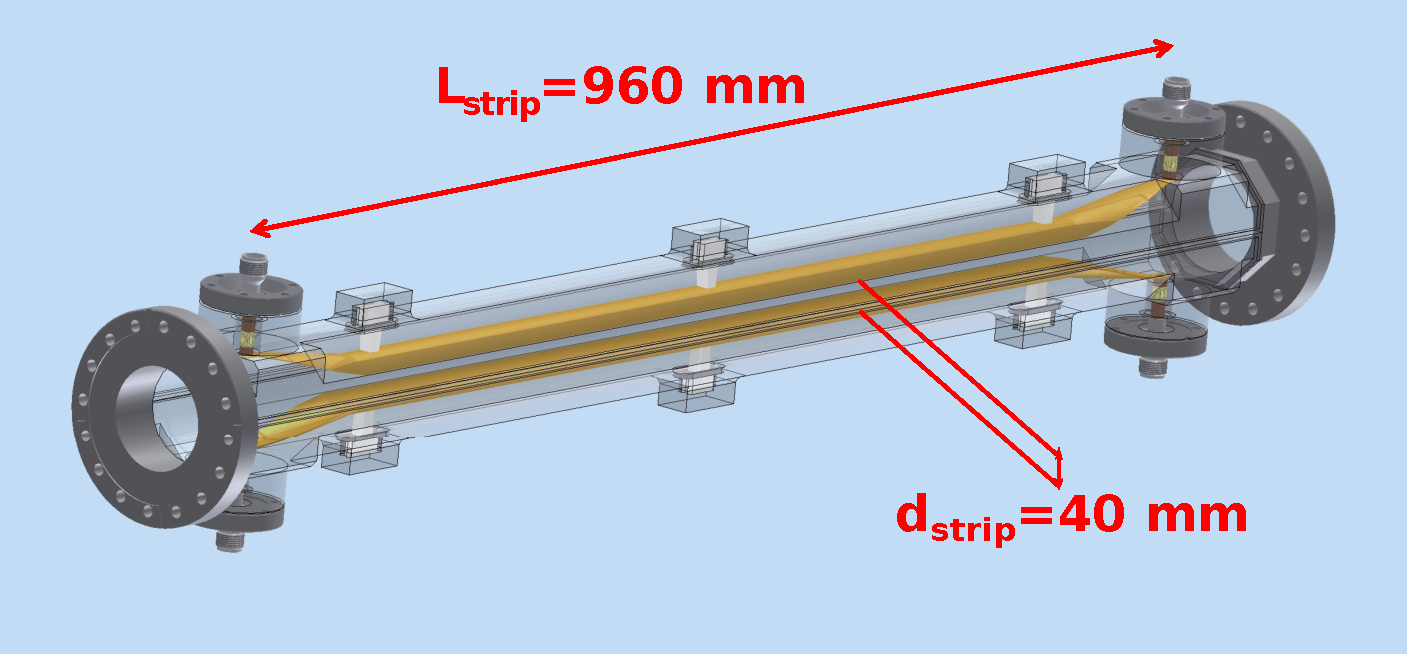
\includegraphics[width=0.8\textwidth]{Figures/optics/kickerSchematic}
  \caption{Technical drawing of the kicker design. The kicker is shown in a vertical orientation with the strips on the top and bottom. When installed in the beam line the kicker is oriented with the strips on the left and right, in order to create a horizontal electric field between the strips.}
  \label{f:kickerSchematic}
\end{figure}

At each end of each strip there is a transition to a 50~\(\mathrm{\Omega}\) HN-type connector. A voltage is applied to the downstream end of each kicker strip, with opposite polarity on each side, for example \(+V\) to the left strip and \(-V\) to the right strip. The voltage is produced by the amplifier discussed in Section~\ref{s:amplifierSetup}, and the voltage leaving the upstream ends of the kicker strips is also terminated back at the amplifier. The applied voltage \(V(t)\) creates a horizontal, position independent, electric field and vertical magnetic field between the strips with related amplitudes as follows \cite{byrdKicker}:
\begin{eqnarray}
E_x &\sim& V(t) \\
B_y &\sim& \frac{V(t)}{c}
\end{eqnarray}
Where \(c\) is the speed of light. By the Lorentz force an electron in the beam propagating with speed \(v\) from the upstream end of the kicker to the downstream end (in the opposite direction to the voltage applied to the strips) experiences the following horizontal force \cite{byrdKicker}:
\begin{equation}
F_x = e(E_x + vB_y) \sim e(1+\beta)V(t) \sim 2eV(t)
\end{equation}
Where \(e\) is the charge of an electron and \(\beta = v/c\). The final expression holds for an ultra-relativistic particle where \(\beta \simeq 1\), which is true for the CTF3 beam. In this case the forces resulting from the electric and magnetic fields have the same magnitude and direction. If the voltage were applied to the upstream end of the strip rather than the downstream end, the magnetic field would be in the opposite direction and the resulting electric and magnetic forces would cancel. 

With the voltage correctly applied to the downstream end of the strips the force is as above and the kicker imparts a horizontal deflection to the beam. The kicker design gives a horizontal deflection of 1~mrad for an applied voltage of \(\pm1.26~kV\) to each strip \cite{kickerIPAC11}, assuming the CTF3 beam energy of around 135 MeV. This value together with the peak voltage output from the amplifier and the optics of the TL2 chicane (as described below) defines the maximum phase offset that can bwe corrected by the PFF system (Section~\ref{ss:corrRange}).



\newsection{tl2}{TL2}

The transfer line TL2 at CTF3 transports the beam from the exit of the combiner ring to the experimental area CLEX (see Figure~\ref{f:ctfLayout}). The whole line is approximately 45~m long and contains both vertical and horizontal chicanes to align the outgoing combiner ring beam line to the CLEX entrance. The PFF system attempts to correct the beam phase using the horizontal chicane at the end of TL2, where the two kickers are installed. Further details of the design of TL2 can be found in \cite{tl2}.

\afterpage{\begin{landscape}
\begin{figure}
  \centering
  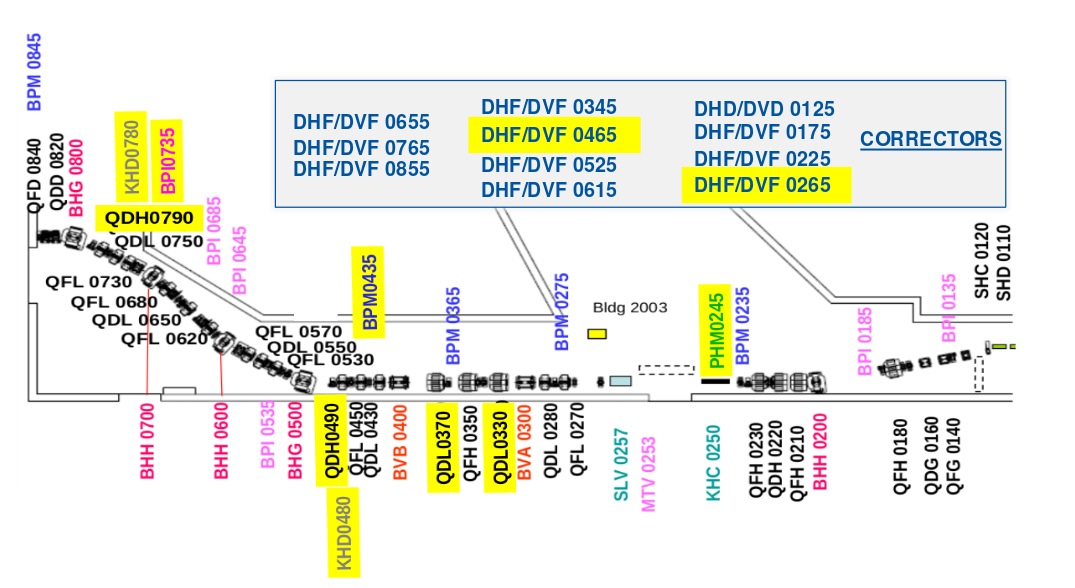
\includegraphics[width=\hsize]{Figures/optics/newTL2Lattice}
  \caption{New TL2 lattice for PFF. Changes highlighted yellow. Adapted from \cite{tl2Layout}}
  \label{f:newTL2Lattice}
\end{figure}
\end{landscape}}


The diagram in Figure~\ref{f:newTL2Lattice} shows a birds-eye view of the TL2 line and the lattice of the line. To interpret the diagram it is useful to introduce the device naming convention at CTF3. Devices have names of the form:
\begin{center}
[CC].[QF][D][0840]
\end{center}
The first two letters refer to the section of the machine, with the prefix CC used for TL2. These are not included in the diagram to improve readability. In Chapters~\ref{c:phaseMons}~and~\ref{c:phasePropagation} the prefix CT is used to refer to the CT-line after the linac and transfer line TL1 prior to the combiner ring. The second group of letters refer to the type of device, the main ones being QF and QD for horizontally focusing and defocusing quadrupoles, BH and BV for horizontal and vertical dipoles, BP for beam position monitors (BPMs) and DH and DV for horizontal and vertical corrector magnets. The last letter indicates the type of that device, with four different designs of quadrupole used along the TL2 line (G-type, H-type, L-type and D-type), for example. The four final numbers indicate the position of that device along the line, in ascending order from the beginning to the end of the line.

The horizontal chicane of interest for the PFF system starts at the dipole CC.BHG0500 and ends at the dipole CC.BHG0800. The first (500) and last (800) dipoles bend the beam through \(+31^\circ\) and \(-31^\circ\) respectively. Inside the chicane there are two further dipoles of a different type -- CC.BHH0600 and CC.BHH0700, which deflect the beam through \(+17^\circ\) and \(-17^\circ\) respectively. Some details on the differences between the two types of dipole are given in Section~\ref{ss:modelErrorSources}. The resulting overall chicane has a ``dog leg'' shape around 12~m in length, with three straight sections around 4~m in length between the bending magnets. Each straight section contains a triplet of quadrupoles and either one (in the first and last sections) or two (in the middle section) BPMs (of the BPI type \cite{bpi}). Although the quadrupoles are labelled as horizontally focusing or defocusing the polarity of the current sent to each can be reversed so that it focuses in the opposite plane. The F or D labels refer to whether the magnet is horizontally focusing or defocusing when a positive current is sent to the quadrupole.

Other features along the TL2 line that are important for the derivation of optics seen later in this chapter include the vertical chicane and two long drift spaces without focusing elements. The vertical chicane starts and ends at CC.BVA0300 and CC.BVB0400 respecitvely, and contains a triplet of quadrupoles. Between the quadrupole CC.QFD0840 (the last shown in the diagram) and CC.QFL0910, there is a long drift space of around 4~m with no focusing elements as the beam pipe passes through in to the neighbouring building where the CLEX area is located. Between the quadrupole CC.QFH0230 and CC.QFL0270 there is another long drift space, around 7~m. The Twiss beta and alpha functions entering these long drifts must be carefully chosen to avoid unrecoverable growth in the beam size.

[TODO: picture of TL2/chicane]

\subsection{Integration of PFF Hardware}
\label{ss:tl2PFFIntegration}

Due to building and cost constraints the PFF prototype had to make use of the pre-existing layout of the TL2 horizontal chicane, with only minor modifications possible to accommodate the PFF hardware. These changes are highlighted in yellow in Figure~\ref{f:newTL2Lattice}.

\begin{figure}
  \centering
  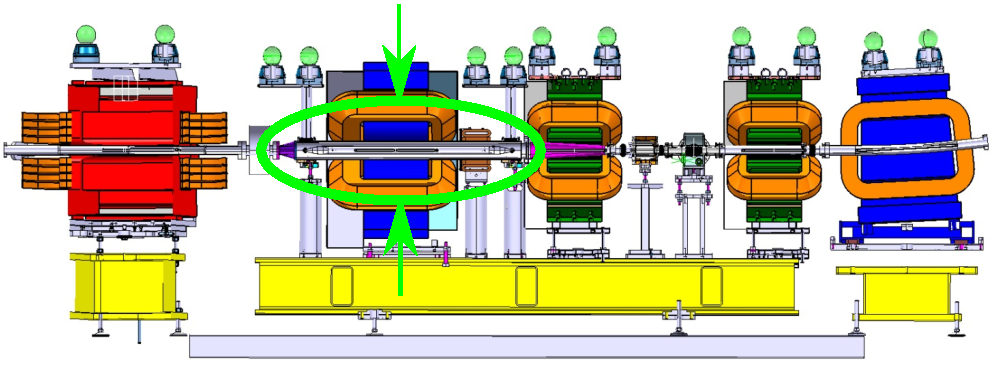
\includegraphics[width=\textwidth]{Figures/optics/kickerInsideQuad}
  \caption{Schematic of the installation of the first kicker inside the quadrupole CC.QDH0490 (blue) before the first dipole in the chicane CC.BHG0500 (red). The kicker also passes through the aperture of the corrector CC.DHF0465 (brown) before the quadrupole \cite{kickInQuad}.}
  \label{f:kickerInsideQuad}
\end{figure}

As the chicane was already densely packed with quadrupoles and other devices the integration of the two kickers was not straightforward. To maintain the functionality of the lattice quadrupoles could not be removed, and thus instead the kickers have been installed inside wide aperture `H-type' quadrupoles \cite{tl2Magnets}. Two `L-type'  quadrupoles \cite{tl2Magnets} (now CC.QDL0330 and CC.QDL0370) from the horizontal chicane were swapped with two `H-type' quadrupoles (now CC.QDH0490 and CC.QDH0790) from the vertical chicane. The two PFF kickers, CC.KHD0480 and CC.KHD0780, are then installed inside the aperture of these quadrupoles, prior to the first and last dipole of the horizontal chicane. In addition, two magnetic correctors (now CC.DHF0465 and CC.DHF0765) were installed around the PFF kickers to facilitate a complementary, large range but low bandwidth, slow phase correction \cite{jackLCWS14}. A schematic of the installation of the first kicker inside the quadrupole and corrector is shown in Figure~[REF]. The kicker CC.KHD0480 will also be referred to as the first kicker (or K1), and CC.KHD0780 as the second kicker (or K2).

Apart from the quadrupoles and correctors two BPMs (now CC.BPI0435 and CC.BPI0735) had to be moved slightly to vacate the area now occupied by the kickers. Finally, a slot near the start of TL2 (CC.PHM0245) was reserved for the installation of an additional phase monitor to verify the beam phase prior to the correction. Eventually this was not necessary and has not been pursued as the 2~cm aperture of the phase monitors (Section~\ref{s:phaseMonDesign}) compared to the 4~cm aperture of the neighbouring beam pipe would have created beam setup difficulties for normal operation at CTF3 \cite{piotrPriv}.

\newsection{tl2OpticsReqs}{TL2 Optics Constraints}

To take in to account the changes made to the TL2 lattice new optics were needed. This section summarises the various optics constraints that must be met in TL2. These can be split in to two types -- the nominal optics constraints, required to recover the same (or similar) beam conditions as before the changes, and the new optics constraints for operation of the PFF system, required to create the desired phase shifting behaviour in the chicane.

\subsection{Nominal Optics Constraints}
\label{ss:nominalOpticsReqs}

The nominal optics constraints are mostly put in place to minimise the transverse beam size along the line by restricting the magnitude of the dispersion and twiss functions. The final constraints, on the \(R_{56}\) transfer matrix coefficient, relates to the longitudinal stability of the beam.

\subsubsection{Dispersion}

The trajectory of a particle through a dipole depends on its energy, with lower energy particles following a smaller radius of curvature and high energy particles a larger radius. After a dipole the orbit of a particle though the following elements therefore depends on its energy. This effect is characterised using the horizontal and vertical dispersion, \(D_x\) and \(D_y\), which are defined as follows (considering only the energy component of the beam orbit):
\begin{eqnarray}
x(s) &=& D_x(s)\left(\frac{\Delta p}{p}\right) \\
y(s) &=& D_y(s)\left(\frac{\Delta p}{p}\right)
\end{eqnarray}
The dispersions \(D_x(s)\) and \(D_y(s)\) vary along the lattice and are equivalent to the transfer matrix coefficients \(R_{16} = D_x\) and \(R_{36} = D_y\). 

Optics are usually created so that there is no dispersion (\(D_{x} = D_{y} = 0\)) in straight sections. However, inside chicanes and rings the dispersion can never always be zero. To give zero dispersion in the straight sections the dispersion must therefore be closed at the exit of all bending sections. Dispersion closure means that both the dispersion and its derivative (\(D_x' = \mathrm{d}D_x/\mathrm{d}s\), and \(D_y' = \mathrm{d}D_y/\mathrm{d}s\)) are zero at the exit from the chicane or ring. In TL2 this condition applies after the bend CC.BHH0200 at the start of the line and at the exit of the horizontal chicane (CC.BHG0800) for the horizontal dispersion, and at the exit of the vertical chicane (CC.BVB0400) for the vertical dispersion.

Within the bending sections the magnitude of the dispersion should be kept as small as possible whilst meeting the other optics constraints. At CTF3 there can be peak-to-peak energy offsets at around the \(\pm1\%\) level \cite{CTF3}. Dispersion is then usually the largest contribution to the beam size, with a dispersion of 1~m giving excursions up to \(\pm1\)~cm in individual particle orbits, for example. The diameter of the beam pipe in bending sections at CTF3 is 10~cm in most cases, as opposed to 4~cm in straight sections, in order to minimise the effects of dispersion dependent beam size growth on the beam transport \cite{CTF3}. However, the second kicker installed in the chicane for the PFF system (CC.KHD0780) only has the normal 4~cm aperture (2~cm radius).  Dispersion around the second kicker must therefore be kept well below 2~m to avoid losing a fraction of off-energy particles on the kicker strips.

\subsubsection{Twiss Functions}

%Normalised emittance around 150 micrometres (best case?)
%Gamma is 135 MeV/0.5 MeV = 270 at CTF3
%Normalised emittance is beta*gamma*emittance
%real emittance is 0.5555 micrometres
%50~m beta function gives around +/- 0.5 cm beam size

The twiss beta functions define the energy independent component of the transverse beam size and the alpha functions define the rate of change of the beta function along the line, as discussed in Section~\ref{s:opticsIntro}. The transverse beam size at any point in the lattice is related to the beta function and emittance via the relationship \(\sqrt{\beta_x(s)\epsilon_x}\) (and the vertical equivalent). At CTF3 the beam emittance is usually around 0.5~\(\mathrm{\mu m}\), but may be up to a factor two larger than this in the horizontal plane depending on the beam setup \cite{davideThesis}. With an emittance of 0.5~\(\mathrm{\mu m}\) a beta value of 50~m at one point in the lattice corresponds to a transverse beam size of 0.5~cm at that location, for example. The beta and alpha functions should be kept as small as possible to minimise the beam size along the line. Beta is usually kept below 50~m, but values up to 100~m can be accepted \cite{piotrPriv}. As mentioned previously there are long drift spaces with no focusing elements at the start and end of TL2, and it is most difficult to maintain low beta and alpha values following these regions.

At the start of TL2 the initial values of the twiss parameters are also constrained by the optics of the combiner ring. In other words, the beta and alpha values at the start of TL2 should be the same as the beta and alpha values at the exit of the combiner ring. This avoids discontinuities between sections in the complete CTF3 optics. The TL2 optics have usually been matched (Section~\ref{s:matchedOptics}) starting from CC.QFH0210, and the required initial conditions at this location are summarised in Table~\ref{t:tl2InitTwiss}.

\begin{table}
  \begin{center}
    \begin{tabular}{|c c|}
	   \hline
       Parameter & Value \\
       \hline
       \(\beta_x\) & 7.26~m\\
	   \(\beta_y\) & 5.90~m\\
	   \(\alpha_x\) & -4.84\\
	   \(\alpha_y\) & -1.27\\
	   \hline
    \end{tabular}
    \caption{Initial twiss parameters for the TL2 line, taken at the entrance to CC.QFH0210.}
  	\label{t:tl2InitTwiss}
  \end{center}
\end{table}

\subsubsection{R56}

The dispersion describes how the transverse orbit of a particle is changed by its energy in bending sections as already discussed. These differences can also change the longitudinal path length of the particle's trajectory, thereby shifting the particle's phase (described by the time \(t\), the fifth coordinate in the matrix formalism). This effect is described by the transfer matrix coefficient \(R_{56}\):
\begin{equation}
t_{f} = t_{i} + R_{56}\left(\frac{\Delta p}{p}\right)
\end{equation}

The \(R_{56}\) value between the entrance and exit of all bending sections at CTF3 is nominally zero so that there is no transformation of energy jitter in to phase jitter. In TL2 this places the constraints for \(R_{56}\) to be zero between the entrance and exit of the vertical chicane (CC.BVA0300 to CC.BVB0400) and between the entrance and exit of the horizontal chicane (CC.BHG0500 to CC.BHG0800).

\subsection{PFF Optics Constraints}
\label{ss:pffOpticsReqs}

All the additional PFF optics constraints place requirements on the transfer matrix coefficients between the two kickers, from the exit of the first kicker to the entrance of the second kicker. There are two sets of constraints, one to maximise the correction range of the PFF system and the other to ensure the PFF system does not degrade the orbit stability of the beam after the chicane.

\subsubsection{Correction Range}

The PFF system clearly requires the path length between the two kickers to depend on the applied kick. This difference in path length dependent on the voltage applied to the kickers is what shifts the time or phase of the beam to form the correction. The transfer matrix coefficient that relates the time variable to the deflection induced by the kickers is \(R_{52}\):
\begin{equation}
t_{K2} = t_{K1} + R_{52}x_{K1}'
\end{equation}
Where \(t_{K1}\) and \(t_{K2}\) are the time offset of the particle at the exit of the first kicker and at the entrance to the second kicker respectively. \(x_{K1}\) is the divergence at the exit of the first kicker resulting from the applied kick. MADX uses units of metres for its `time' variable \cite{madx}. To convert these distances in to 12~GHz degrees they must be multiplied by the constant factor \(360/\lambda_{\mathrm{12GHz}}\), where \(\lambda_{\mathrm{12GHz}} = 2.5\)~cm is the 12~GHz wavelength. Directly in terms of phase (in degrees) the equation above therefore becomes:
\begin{equation}
\phi_{K2} = \phi_{K1} + R_{52}\left(\frac{360}{\lambda_{\mathrm{12GHz}}}\right)x_{K1}'
\end{equation}
Where \(\phi_{K2}\) is the phase at the entrance to the second kicker (the corrected phase) and \(\phi_{K1}\) is the initial uncorrected phase at the exit of the first kicker. The maximum value of \(x_{K1}'\) is fixed by the peak voltage output from the kicker amplifiers and the design of the kickers themselves. To obtain the largest possible correction range for the PFF system given the parameters of the hardware, the \(R_{52}\) transfer matrix coefficient should be as large as possible. For example, with \(R_{52} = 1\)~m and a maximal kick of \(x_{K1}' = \pm 1\)~mrad, the correction range of the PFF system would be \(\pm 14.4\)~degrees.

The path length difference in the chicane largely results from differing trajectories in the dipoles. In this way it is somewhat analogus to the dispersion, which describes the energy dependent difference in beam orbit after dipoles. This has the unfortunate consequence of leading to optics with high \(R_{52}\) values also tending to have high peak dispersion values in the chicane. The PFF optics must therefore be a compromise that achieves a reasonable correction range whilst keeping the dispersion small enough to avoid beam losses in the chicane.

\subsubsection{Orbit Closure}

The PFF system should not change the beam orbit after the chicane, which means the beam position and divergence after the second kicker must be independent of the applied kicks. In other words, the second kicker must close the horizontal orbit bump created by the first kicker. To understand the further constraints this places on the optics the position, \(x_{K2}\), and divergence \(x_{K2}'\) of the beam at the entrance to the second kicker will be considered first. These can be expressed as:
\begin{eqnarray}
x_{K2} &=& R_{11}x_{K1} + R_{12}x_{K1}' \\
x_{K2}' &=& R_{21}x_{K1} + R_{22}x_{K1}'
\end{eqnarray}
Where \(x_{K1}\) and \(x_{K1}'\) are the position and divergence at the exit of the first kicker, and \(R_{11}\), \(R_{12}\), \(R_{21}\) and \(R_{22}\) are transfer matrix coefficients for the optics between the exit of the first kicker and the entrance to the second kicker. The beam position at the exit of the first kicker is proportional to the applied kick:
\begin{equation}
x_{K1} = m x_{K1}'
\end{equation}
Here \(m\) is a constant that depends on the properties of the kicker and also on the strength of the quadrupole CC.QDH0490 within which the kicker is installed (Section~\ref{ss:tl2PFFIntegration}). Substituting this expression in to the equations for \(x_{K2}\) and \(x_{K2}'\) gives:
\begin{eqnarray}
x_{K2} &=& \left(R_{11} + \frac{R_{12}}{m}\right)x_{K1} \\
x_{K2}' &=& (m R_{21} + R_{22})x_{K1}'
\end{eqnarray}
As stated \(x_{K2}\) and \(x_{K2}'\) are defined above at the entrance to the second kicker. The requirement for the PFF chicane optics is that the position and divergence at the exit of the second kicker are zero independent of the applied kicks. However, a derivation of the exact expression for the optics requirements between the kickers in order to close the orbit at the exit of the second kicker is complicated by the fact that the quadrupole around the second kicker, CC.QDH0790, can have a different strength to the quadrupole around the first kicker. 

For the purpose of the discussion here the simplified case where CC.QDH0790 has the same strength but opposite polarity (focuses in the opposite plane) as CC.QDH0490 will be considered. The ideal case where the two kickers can be powered with the same magnitude voltage but opposite polarity is also assumed. With these conditions, the second quadrupole/kicker effectively have precisely the opposite effect on the beam as the first quadrupole/kicker. To close the orbit after the second kicker the position and divergence at the entrance to the second kicker must therefore meet the following criteria:
\begin{eqnarray}
x_{K2} &=& -x_{K1} \\
x_{K2}' &=& x_{K1}'
\end{eqnarray}
Comparing these two expressions to the previously derived equations for \(x_{K2}\) and \(x_{K2}'\) then yields the following optics constraints:
\begin{eqnarray}
R_{11} + \frac{R_{12}}{m} &=& -1  \label{e:orbClosConst1} \\
m R_{21} + R_{22} &=& +1 \label{e:orbClosConst2}
\end{eqnarray}
There are many possible solutions to these expressions, with the simplest example being \(R_{11} = -1\), \(R_{12} = 0\), \(R_{21} = 0\) and \(R_{22} = 1\). However, the optics matching (Section~\ref{s:matchedOptics}) allows the quadrupoles CC.QDH0490 and CC.QDH0790 to have different strengths. MADX is then used to model the actual beam orbit in the chicane and the figure of merit is for the simulated orbit to be closed after the second kicker, rather than for the above constraints to be met. Nevertheless, the optics eventually created do satisfy Equations~\ref{e:orbClosConst1}~and~\ref{e:orbClosConst2} within several percent (Section~\ref{ss:tl2PFFOptics}).

%First assuming a simplified case of zero length kickers (with only the divergence changing in the kicker and not the beam position), the position \(x_{K2}\), and divergence, \(x_{K2}'\), of the beam at the entrance to the second kicker can be expressed as:
%\begin{eqnarray}
%x_{K2} &=& R_{12} x_{K1}' \\
%x_{K2}' &=& R_{22} x_{K1}'
%\end{eqnarray}
%Where \(x_{K1}\) and \(x_{K1}'\) are the position and divergence at the exit of the first kicker, and \(R_{12}\) and \(R_{22}\) are transfer matrix coefficients for the optics between the exit of the first kicker and the entrance to the second kicker. The position and divergence after the second kicker, \(x_f\) and \(x_f'\) are then given by:
%\begin{eqnarray}
%x_{f} &=& x_{K2} \\
%x_{f}' &=& x_{K2}' \mp x_{K1}'
%\end{eqnarray}
%The equation for the divergence assumes the ideal case where both kickers are powered with the same magnitude voltage. Inserting the expressions for \(x_{K2}\) and \(x_{K2}'\) above places the optics requirements \(R_{12} = 0\) and \(R_{22} = \pm 1\) to ensure orbit closure after the second kicker.

\newsection{opticsMeas}{TL2 Optics Measurements}

As seen above there are many optics constraints in TL2 that must be met both to ensure that the beam can be transported efficiently in to the CLEX area as well as to obtain the desired behaviour in the horizontal chicane for the PFF system. MADX can be used to create optics that meet these criteria (Section~\ref{s:matchedOptics}), but they will be of no use if the model of TL2 does not accurately desribe the actual characteristics of the line. As such, a series of measurements has been taken to determine and improve the accuracy of the TL2 MADX model. Measurements of this type had not previously been completed for the TL2 line at CTF3, thus any errors identified in the model are not limited to only the hardware changes made for the PFF system.

\subsection{Method}
\label{ss:opticsMethod}

The TL2 line includes 12 magnetic correctors, as shown in Figure~\ref{f:newTL2Lattice} (plus one at the end of TL2 in the CLEX area, which is not shown in the figure). An electric current can be applied to horizontal or vertical coils on the corrector, creating independently adjustable horizontal and vertical fields that deflect the beam. The primary purpose of the correctors is to compensate differences in beam orbit resulting from small misalignments of devices along the line. However, they can also be used to test the accuracy of the TL2 model.

Measurements were taken in which the current applied to one of the correctors was changed, causing the beam to be deflected on to a new trajectory along the rest of the line. The new orbit is observed in the BPMs downstream of the corrector, with a total of 12 BPMs in TL2 (also shown in Figure~\ref{f:newTL2Lattice}). The position offset in each BPM depends on the transfer matrix between the corrector and that BPM, and therefore on the focusing properties of all the magnetic elements between the corrector and the BPM. By deflecting the beam with each corrector along the line, and in both planes, the response of the whole line as well as individual parts of the line can be determined.

The same process can then be repeated in the MADX model, applying a current to one of the correctors and creating a simulated deflected orbit. All the BPMs are included in the model, allowing the real measured position in each BPM to be compared to the simulated position from the MADX model. Any difference between the two highlights inaccuracies in the modelled properties of the TL2 lattice.

\subsection{Results with Original MADX Model}
\label{ss:opticsResults}

Figures~\ref{f:modelOriginalH}~and~\ref{f:modelOriginalV} show an example of the results obtained with the original version of the TL2 MADX model, in the horizontal and vertical planes respectively. One of the first correctors in TL2, CC.DHF0175 (or the equivalent CC.DVF0175 in the vertical plane), is used, so the results are sensitive to errors in the model along the full length of the line. Three lines are shown in each figure -- the red line labelled ``Measurement'' corresponds to the actual measured position in the BPMs, the dashed blue line ``Model'' shows the simulated position in the BPMs from MADX, and the final black line ``Full'' shows the simulated MADX orbit propagated through all elements along the line (not restricted to only the BPM positions). In a perfect model of the line the blue ``Model'' and red ``Measurement'' lines would be identical.

In the horizontal plane there is good agreement between the model and the measurement in the three BPMs following the corrector (up until CC.BPM0275). After this point the response in the model is clearly completely different to the measurement. For example, the measured position shifts by 10~mm between CC.BPM0275 and CC.BPM0365 in the measurement, but only 6~mm in the model. Towards the end of the line the model is close to being the inverse of the measurement. There is also poor agreement between the model and the measurement in the vertical plane, with a large difference already visible at CC.BPM0275 in this case. The peak-to-peak vertical orbit offset in the model is roughly a factor two larger than the measurement.

\begin{figure}
  \centering
  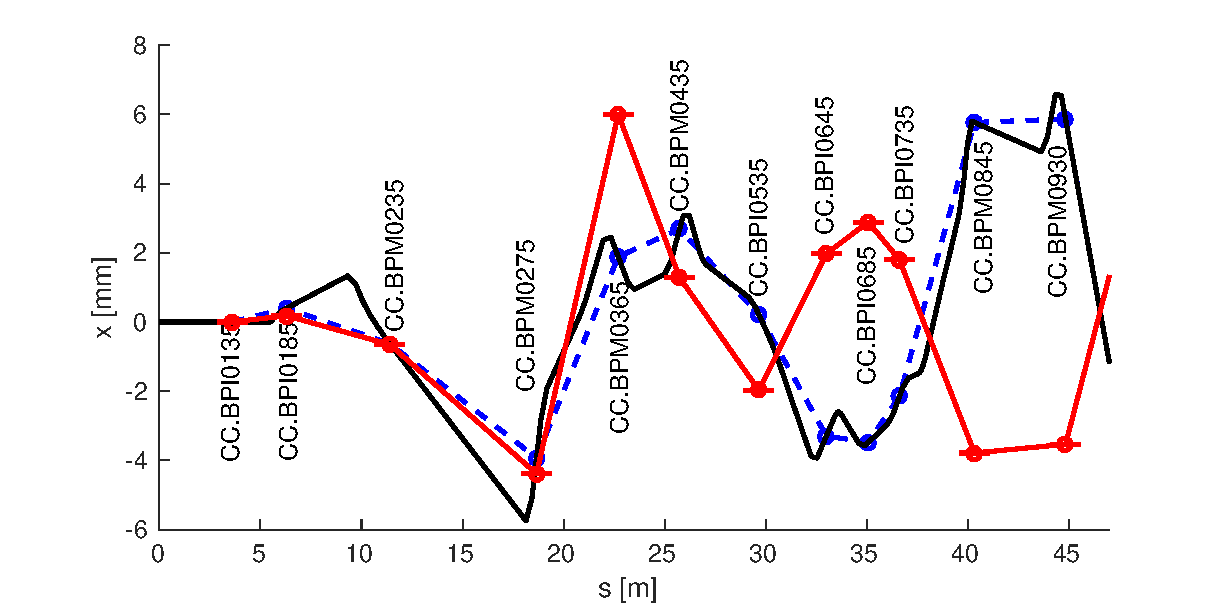
\includegraphics[width=0.9\textwidth]{Figures/optics/modelOriginalH}
  \caption{Horizontal orbit due to a kick from the corrector CC.DHF0175 (red) compared to the expected orbit in the original MADX model of TL2. The black line shows the MADX orbit propagated through all elements along the line, and the dashed blue line the orbit restricted to only the BPM positions.}
  \label{f:modelOriginalH}
  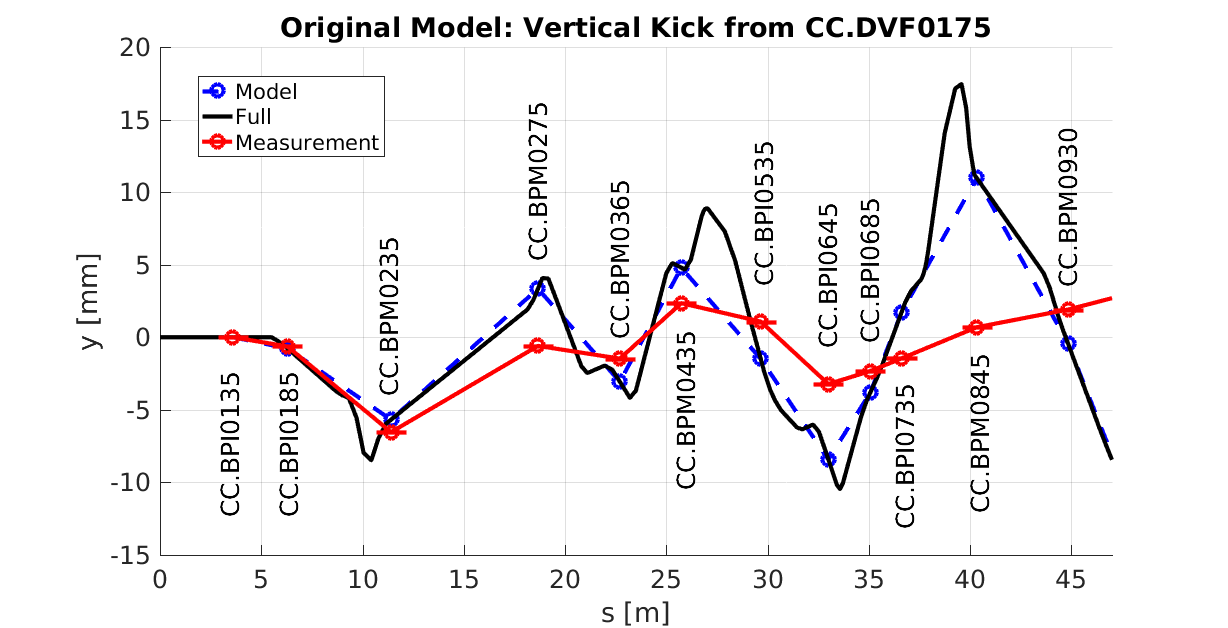
\includegraphics[width=0.9\textwidth]{Figures/optics/modelOriginalV}
  \caption{Vertical orbit due to a kick from the corrector CC.DHF0175 (red) compared to the expected orbit in the original MADX model of TL2. The black line shows the MADX orbit propagated through all elements along the line, and the dashed blue line the orbit restricted to only the BPM positions.}
  \label{f:modelOriginalV}
\end{figure}

\subsection{Sources of Errors in MADX Model}
\label{ss:modelErrorSources}

The results described above immediately demonstrated large discrepancies between the model and the actual response of TL2. Based on previous experience from corrections made to the MADX model for other sections of CTF3 \cite{benOptics} two key areas were identified to investigate to try to improve the model --- the properties of the ``L-type'' quadrupoles in TL2, and the focusing effects from the dipoles in TL2.

\subsubsection{Quadrupole Strengths}
\label{sss:quadStrengths}

16 out of the 27 quadrupoles in TL2 are of the ``L-type'', with labels of the form CC.QDLxxxx or CC.QFLxxxx. This includes all the quadrupoles in the horizontal chicane apart from the two wide aperture ``H-type'' quadrupoles within which the PFF kickers are installed. These quadrupoles were reclaimed from the CELSIUS project in Uppsala, Sweden \cite{celsius}. In the MADX model of TL2 the focusing strength of these magnets, \(K1\) is defined by the following parameters:
\begin{equation}
\mathrm{K1} = \frac{\mathrm{FQL}\times I}{E}
\end{equation}
Where \(\mathrm{FQL} = 31.78\) is a constant defined by the properties of the quadrupole, \(I\) is the current delivered to the quadrupole from its power supply a larger focusing effect) and \(E\) is the beam energy. The \(\mathrm{K1}\) value is analogus to the constant \(k\) in the quadrupole transfer matrix previously seen in Equation~\ref{e:quadTransfer}. This must be multiplied by the 30~cm active magnetic length of the quadrupole to determine the equivalent focal length of the quadrupole.

As the properties of the ``L-type'' quadrupoles were not measured in place at CERN prior to their use in CTF3 there was a large uncertainty on the correct value of \(\mathrm{FQL}\) to use. Changing the \(\mathrm{FQL}\) value was therefore a good candidate to try to reduce errors in the MADX model.

\subsubsection{Dipole Focusing}
\label{sss:edgeFocusing}

Although the primary purpose of dipole magnets is to bend the beam they also give focusing effects that depend on the design of the magnet, and in particular the orientation of the pole faces. The seven dipoles in TL2 can be roughly split in to two types in terms of the focusing effects they are expected to produce --- sector magnets (SBENDs) and rectangular magnets (RBENDs). Figure~\ref{f:sbendrbend} compares the geometry of the pole faces for SBEND and RBEND dipoles. In SBEND magnets the ends of the pole faces are oriented such that the reference trajectory of the beam (black) enters and leaves the magnet perpendicular to the pole face. Alternatively, in RBEND dipoles the pole faces at the entrance and exit of the magnet are parallel to each other. In this case the reference trajectory forms an angle \(\theta/2\) with the pole faces, where \(\theta\) is the angle through which the beam is deflected by the magnet \cite{wiedemann}. In TL2 the CC.BHH0200, CC.BHG0500, CC.BHH0600, CC.BHH0700 and CC.BHG0800 dipoles are RBENDs, and the CC.BVA0300 and CC.BVB0400 dipoles are SBENDs \cite{tl2Magnets}.

\begin{figure}
  \centering
  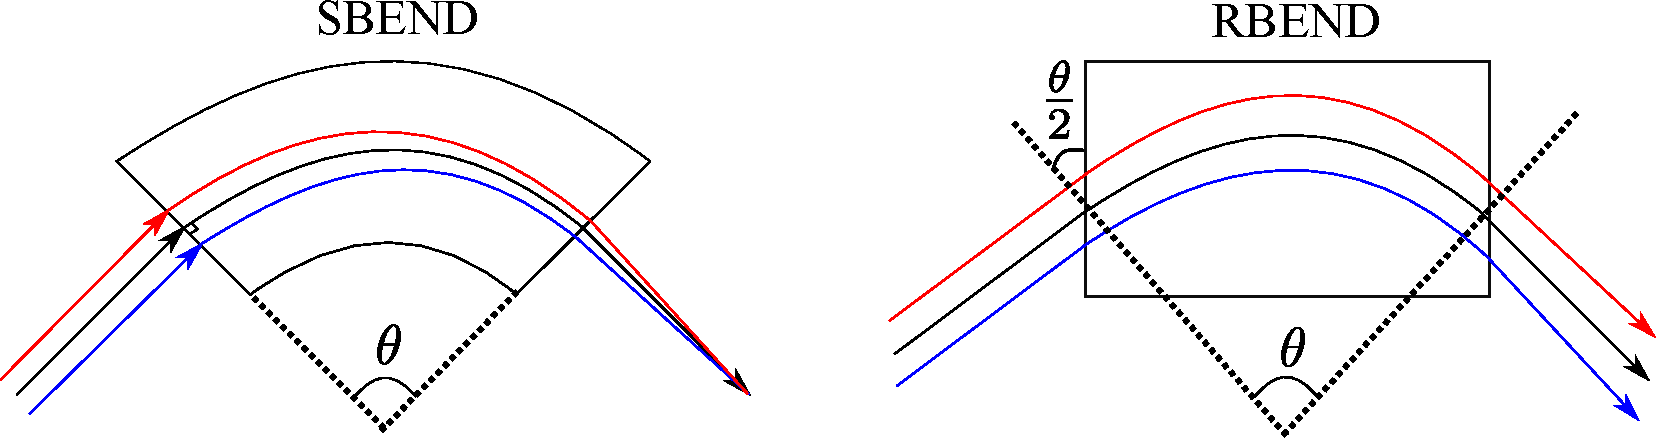
\includegraphics[width=0.9\textwidth]{Figures/optics/sbendrbend}
  \caption{Geometry of SBEND and RBEND dipoles.}
  \label{f:sbendrbend}
\end{figure}

The first focusing effect from dipoles relates to the path length of the beam through the magnet. In SBEND magnets this length depends on the position offset in the (horizontal or vertical) bending plane. Particles entering the magnet experience the dipole field for a longer length on one side of the reference trajectory, and a shorter length on the other side of the reference trajectory, producing a focusing effect in the bending plane. This is also shown in Figure~~\ref{f:sbendrbend}. In RBEND magnets the length of the trajectory is the same for all incoming position offsets, so this focusing effect is not present.

Another way in which dipoles produce focusing effects is via their fringe fields. The fringe fields describe the increase in magnetic field from zero to the peak bending field as the beam approaches the entrance to the dipole, and from the peak field back to zero as the beam leaves the dipole. The extent and rate of increase of the fringe fields depends on the design of the dipole, in particular the pole separation. In MADX the nature of the fringe fields is defined by the variables HGAP, the pole separation, and FINT, which describes the shape of the increase up to the peak field (e.g. linear) \cite{madx}.

In RBEND magnets, where the reference orbit is not perpendicular to the pole faces, the longitudinal position along the trajectory where a particle enters the fringe field linaerly depends on its transverse position offset in the bending plane. This is shown in Figure~\ref{f:sbendrbend}, where the grey shaded areas mark the region of the fringe fields. The red trajectory enters the fringe fields later than the blue trajectory. This creates a position dependent focusing effect which is defocusing in the bending plane and focusing in the other transverse plane, similar to a quadrupole \cite{holzer}. In the ideal case this type of focusing is not present in SBEND magnets.

Finally, higher order field errors in the dipole can lead to further focusing terms. MADX allows a quadrupole field coefficient (K1) to be added to a dipole to model this effect. In other sections of CTF3 it was found that the default MADX parameters did not give a good approximation of the dipole focusing terms \cite{benOptics}. The FINT, HGAP and K1 parameters for each of the 7 dipoles in TL2 are therefore also good candidates to try to correct the  MADX model of TL2.

\subsection{Corrections to MADX Model}
\label{ss:modelCorrections}

By varying the parameters of the dipole focusing and the L-type quadrupole strengths described above it has been possible to find a solution that gives much better agreement between the corrector kick measurements and the expected response in the MADX model. The new values for the parameters do not necessarily represent their true real world characteristics (for example the dipole pole separation), but are rather a set of values that adjusts the simulated MADX focusing in a way that matches the actual behaviour. An iterative process was used, with a mixture of automatic optimisations via algorithms in MATLAB and MADX and manual interventions to drive the calculated adjustments towards a reasonble solution and away from any local minima.

The first adjustment made was to the modelled strength of the L-type quadrupoles. As the majority of quadrupoles along TL2 are of this type the focusing and calculated transfer matrices in the MADX model are very sensitive to any change in their strength. It was quickly determined that the focusing strength of the L-type quadrupoles needed to be increased to improve the agreement between the measurement and the model. Figure~\ref{f:modelCorrQuadH} shows an example of a horizontal kick from the corrector CC.DHF0175 with an optimal increase of \(7\%\) in the L-type quadrupole strength. This can be directly compared to the original model in Figure~\ref{f:modelOriginalH}. By increasing the focusing from the L-type quadrupoles the largest discrepancies between the MADX model and the measurement are removed. In particular the region from inside the vertical chicane (CC.BPM0365) to inside the horizontal chicane (CC.BPI0735) originally showed large differences including sign flips in the horizontal plane. With the adjusted L-type strength these are removed and the agreement is excellent.

\begin{figure}
  \centering
  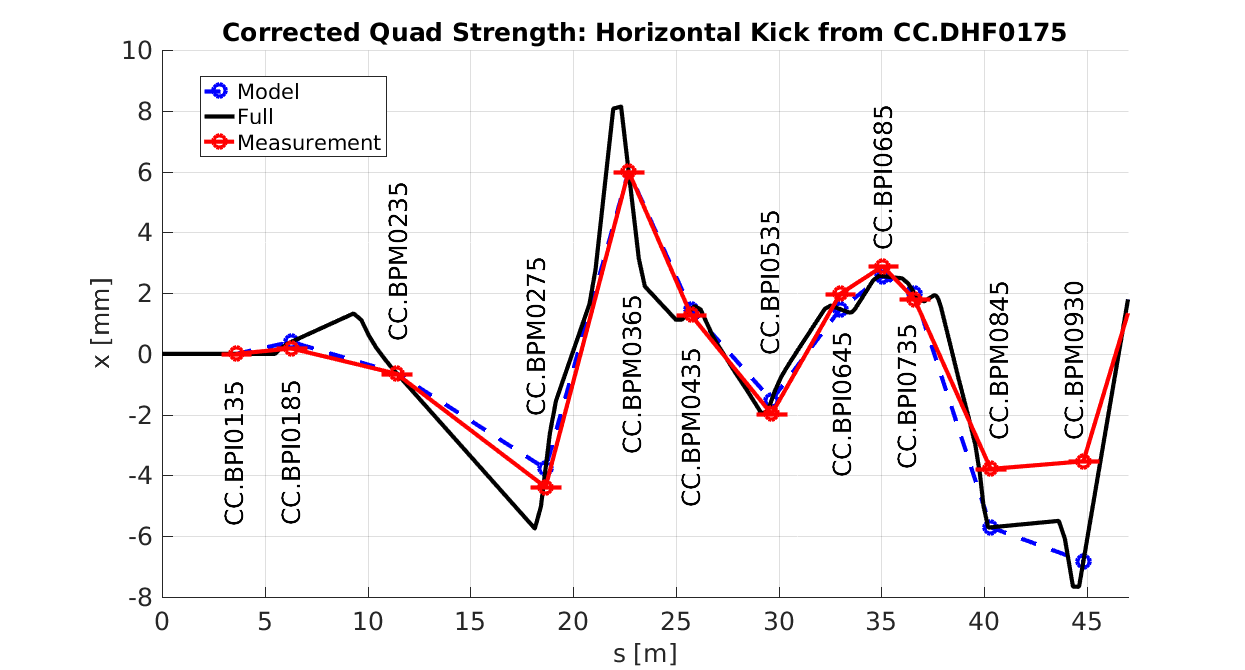
\includegraphics[width=0.9\textwidth]{Figures/optics/modelCorrQuadH}
  \caption{Horizontal orbit due to a kick from the corrector CC.DHF0175 (red) compared to the orbit in the MADX model of TL2 with the L-type quadrupole strengths increased by \(7\%\). The black line shows the MADX orbit propagated through all elements along the line, and the dashed blue line the orbit restricted to only the BPM positions.}
  \label{f:modelCorrQuadH}
\end{figure}

Figures~\ref{f:modelOrigBendV} and \ref{f:modelCorrBendV} then show an example of adjusting the focusing of the four dipoles in the horizontal chicane (the outer 500/800 pair and inner 600/700 pair) to remove remaining differences between the measurement and the model. In this case the beam is kicked from the CC.DVF0525 corrector just after the first dipole in the horizontal chicane, making the measurement insensitive to any optics errors prior to CC.DVF0525 in the line. In both figures the \(7\%\) increase in the L-type quadrupole strength has been applied in the MADX model. With the quadrupole correction in place but no adjustment to the dipole focusing, in Figure~\ref{f:modelOrigBendV}, the simulated orbit has the same overall shape as the measured orbit inside the chicane (up until CC.BPI0735). However, there are still offsets between the two and these eventually lead to a large discrepancy between the model and the measurement still being present in the two BPMs following the chicane (CC.BPIM0845 and CC.BPM0930), which is also seen in Figure~\ref{f:modelCorrQuadH}. 

By adjusting the HGAP, FINT and quadrupole K1 component of the dipoles in the horizontal chicane a solution is found that reduces the difference between the model and the measurement in the chicane, and then also gives much better agreement between the two after the chicane. This is shown in Figure~\ref{f:modelCorrBendV}. Repeating this process with correctors prior to the vertical chicane, and prior to the CC.BHH0200 bend at the start of TL2, yields the focusing parameters for the seven dipoles in the line summarised in Table~\ref{t:tl2ModelChanges}. The largest quadrupolar component of K1 = 0.425~\(\mathrm{m^{-2}}\) for the CC.BHH0600 and CC.BHH0700 dipoles corresponds to a focusing strength of roughly \(2\%\) of a typical quadrupole magnet in TL2.

\begin{figure}
  \centering
  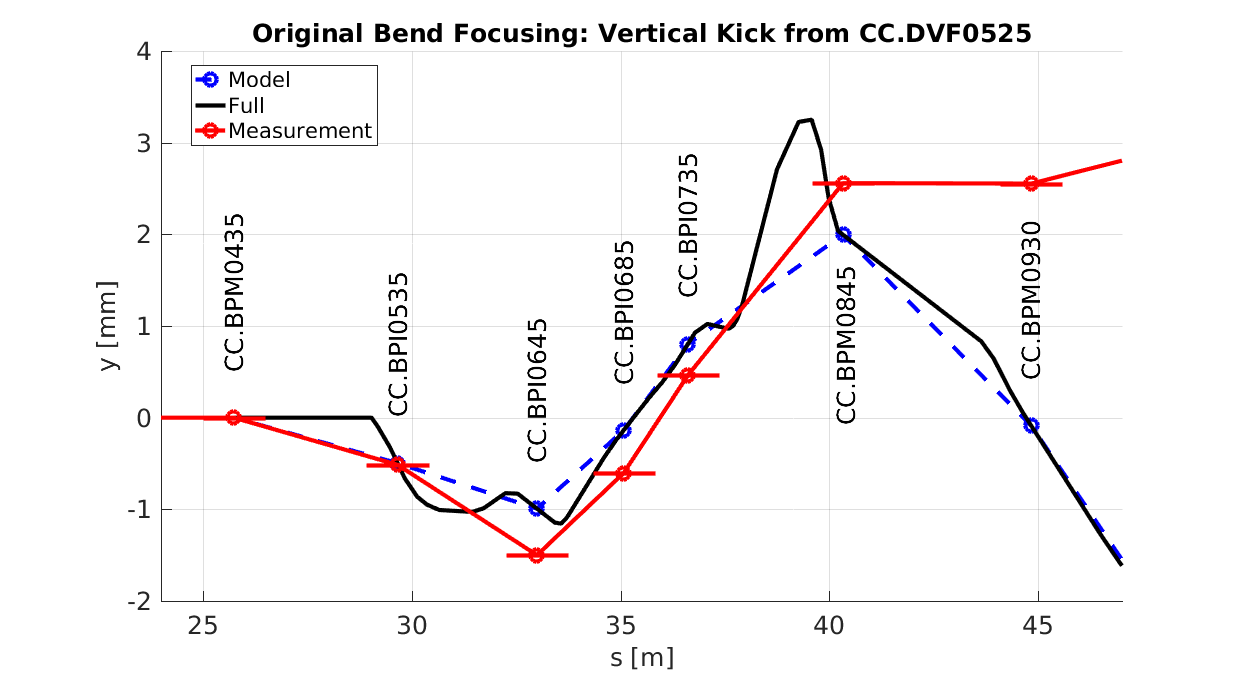
\includegraphics[width=0.9\textwidth]{Figures/optics/modelOrigBendV}
  \caption{Vertical orbit due to a kick from the corrector CC.DVF0525 (red) with the default MADX model of the dipole focusing. The black line shows the MADX orbit propagated through all elements along the line, and the dashed blue line the orbit restricted to only the BPM positions.}
  \label{f:modelOrigBendV}
  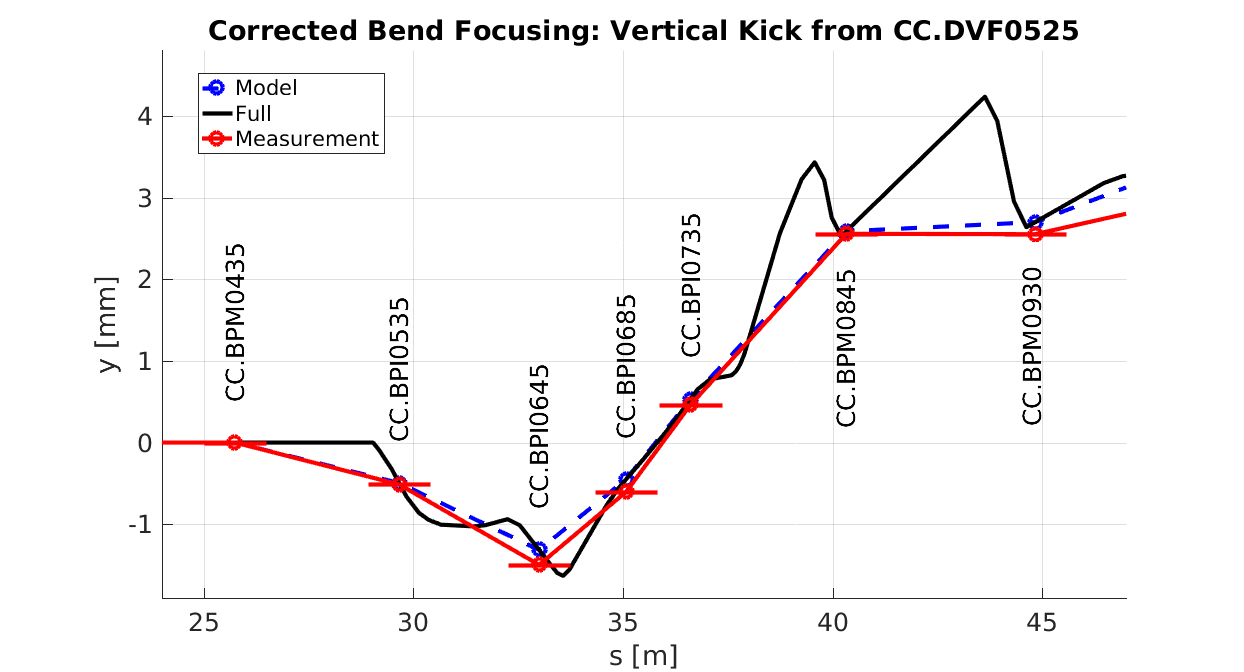
\includegraphics[width=0.9\textwidth]{Figures/optics/modelCorrBendV}
  \caption{Vertical orbit due to a kick from the corrector CC.DVF0525 (red) with the corrected MADX model of the dipole focusing. The black line shows the MADX orbit propagated through all elements along the line, and the dashed blue line the orbit restricted to only the BPM positions.}
  \label{f:modelCorrBendV}
\end{figure}


\begin{table}
  \begin{center}
    \begin{tabular}{|c c c c|}
	    \hline
        Device & Parameter & Original Value & Corrected Value\\ \hline
		CC.BHH0200 & HGAP & 0~m & 0.084~m \\
		 	       & FINT & 0 & 0.79 \\
		           & K1 & 0~\(\mathrm{m^{-2}}\) & 0~\(\mathrm{m^{-2}}\) \\ \hline
		CC.BVA0300   & HGAP & 0~m & 0~m \\
		 	 \&      & FINT & 0 & 0 \\
		CC.BVB0400   & K1 & 0~\(\mathrm{m^{-2}}\) & -0.125~\(\mathrm{m^{-2}}\) \\ \hline
		CC.BHG0500   & HGAP & 0~m & 0.06~m \\
		 	 \&      & FINT & 0 & 0.4 \\
		CC.BHG0800   & K1 & 0~\(\mathrm{m^{-2}}\) & 0.15~\(\mathrm{m^{-2}}\) \\ \hline
		CC.BHH0600   & HGAP & 0~m & 0.06~m \\
		 	 \&      & FINT & 0 & 0.2 \\
		CC.BHH0700   & K1 & 0~\(\mathrm{m^{-2}}\) & 0.425~\(\mathrm{m^{-2}}\) \\ \hline
		L-type Quadrupoles & FQL & 31.78 & 34.03 \\
	   \hline
    \end{tabular}
    \caption{Changes made to the dipole focusing and quadrupole strength parameters in the TL2 MADX model in order to improve the agreement with the kick measurements.}
  	\label{t:tl2ModelChanges}
  \end{center}
\end{table}

Figures~\ref{f:modelCorrectedH}~and~\ref{f:modelCorrectedV} compare the measured horizontal and vertical orbit to the new MADX model of TL2 with all the corrections from Table~\ref{t:tl2ModelChanges} in place. The same corrector, CC.DHF0175, and data are used as for the examples from the original model in Figures~\ref{f:modelOriginalH}~and~\ref{f:modelOriginalV}. The new version of the model is a clear improvement. In both the horizontal and vertical planes the measured and modelled beam orbit now agree along the full length of the line within a small margin of error. With the original MADX model the mean absolute difference between the measured and simulated positions in the ten BPMs following CC.DHF0175 was \(3.9\pm1.0\)~mm in the horizontal plane and \(3.1\pm0.8\)~mm in the vertical plane. The corrected model reduces these differences by an order of magnitude, to \(0.2\pm0.1\)~mm in the horizontal plane and \(0.3\pm0.1\)~mm in the vertical plane.

\begin{figure}
  \centering
  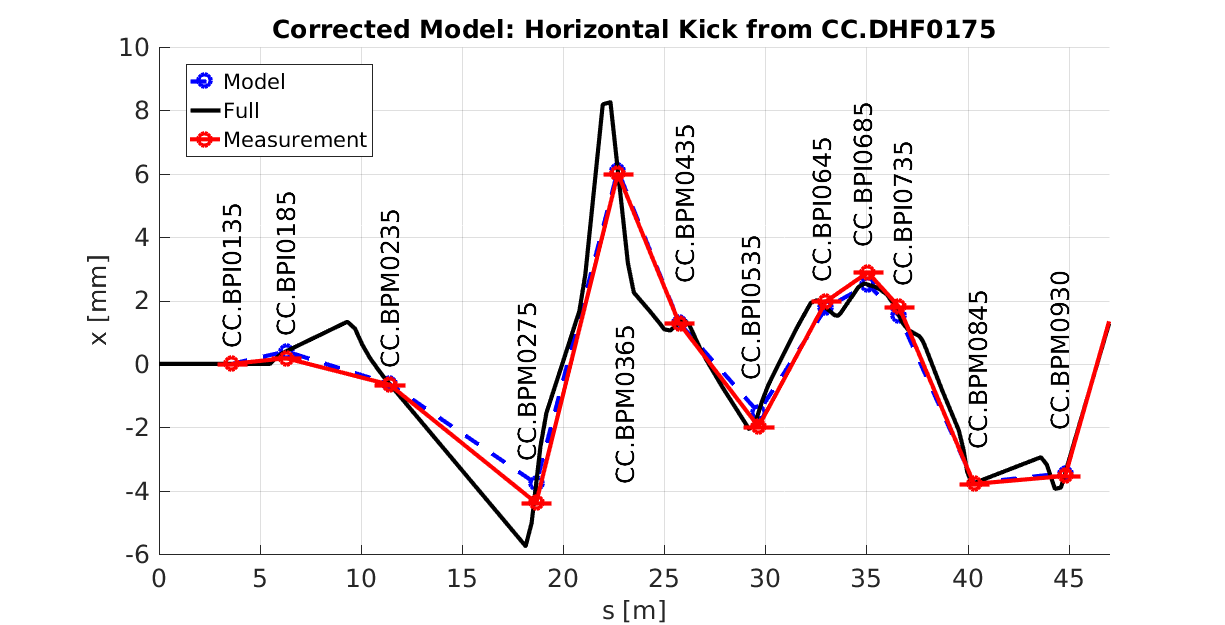
\includegraphics[width=0.9\textwidth]{Figures/optics/modelCorrectedH}
  \caption{Horizontal orbit due to a kick from the corrector CC.DHF0175 (red) compared to the corrected MADX model of TL2. The black line shows the MADX orbit propagated through all elements along the line, and the dashed blue line the orbit restricted to only the BPM positions.}
  \label{f:modelCorrectedH}
  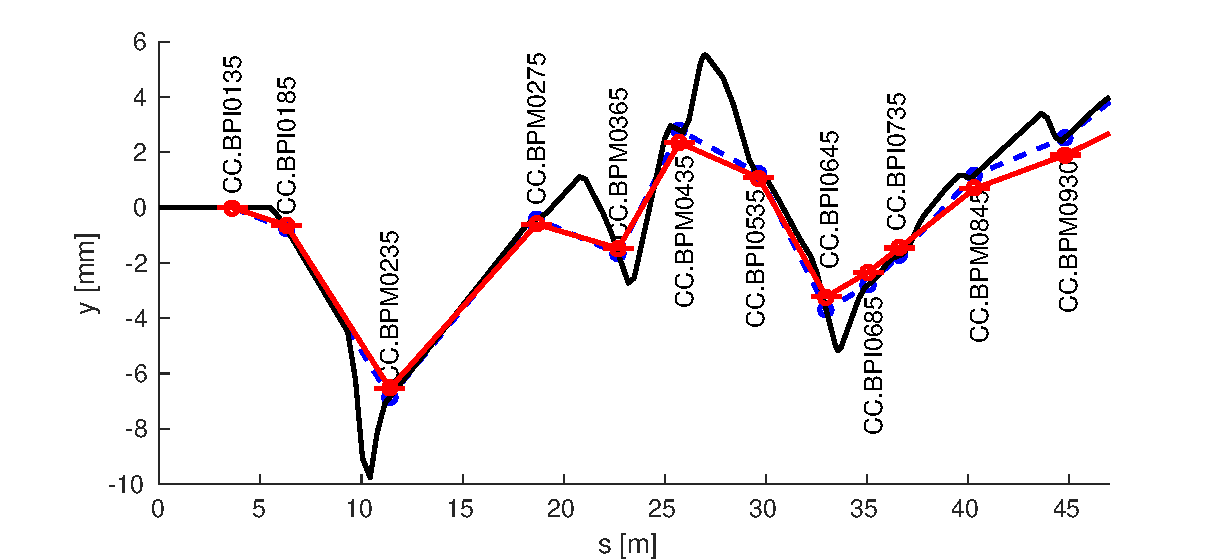
\includegraphics[width=0.9\textwidth]{Figures/optics/modelCorrectedV}
  \caption{Vertical orbit due to a kick from the corrector CC.DVF0175 (red) compared to the corrected MADX model of TL2. The black line shows the MADX orbit propagated through all elements along the line, and the dashed blue line the orbit restricted to only the BPM positions.}
  \label{f:modelCorrectedV}
\end{figure}

\newsection{matchedOptics}{Matched TL2 Optics}

With the corrected MADX model of TL2 in place the new optics for the PFF system were created. The optics were obtained using MADX matching libraries \cite{madx}, in which many desired constraints can be defined for the line (each with its own weight) and then one of several optimisation algorithms can be used to change the quadrupole strengths and derive an optics that meets those constraints. Two sets of optics were created for TL2 -- a nominal set of optics containing only the constraints from Section~\ref{ss:nominalOpticsReqs}, and a set of PFF otpics containing the additional \(R_{52}\) and orbit closure related constraints for the PFF system from Section~\ref{ss:pffOpticsReqs}. Without the additional PFF constraints roughly a factor two smaller maximum dispersion and beta values can be achieved in the nominal optics. However, the beam quality achieved with the PFF optics has been sufficient to use routinely at CTF3 (including for non-PFF running), and so only this optics is documented here.

\subsection{Matching Process}
\label{ss:matchingMethod}

For the purposes of the matching TL2 was split in to three parts -- from the beginning of the line to the exit of the vertical chicane (CC.BHH0210 to CC.BVB0400), from the exit of the vertical chicane to the exit of the horizontal chicane (CC.BVB0400 to CC.BHG0800) and the end of the line (from CC.BHG0800 and in to CLEX). The middle section, containing the PFF kickers and horizontal chicane, is the most critical for the PFF system.

At the beginning of each matching section the initial twiss parameters for that part of the lattice must be defined in MADX. At the start of the first section this is fixed by the properties of the beam leaving the combiner ring (Table~\ref{t:tl2InitTwiss}). The initial and final twiss functions of the middle section containing the horizontal chicane were left as free parameters to allow the greatest degree of flexibility for meeting the constraints in the chicane. The optics for the middle section is therefore created first, with the resulting initial and final twiss parameters forming additional matching constraints that must be met at the end of the first section and the start of the final section.

Suitable initial values for the quadrupole strengths (defined by the current sent to each quadrupole from its power supply) must also be chosen to ensure the matching algorithms can converge to a good solution in a reasonable amount of time. For this purpose the currents from the prior optics for TL2 (before the modifications for the PFF system and the model corrections) were used. 

To accurately simulate the effect of a kick applied at the PFF kickers they must be modelled together with the quadrupoles within which they are installed but this can not be directly defined in MADX. Instead the quadrupole definition in MADX has been split in to quarters, with zero length kicker elemnets inserted between each quadrupole quarter \cite{piotrPriv}. Each kicker element provides a quarter of the angular deflection of the complete kicker. This allows the focusing effect of the quadrupole on the applied kick to be approximated.

All the constraints for each section (taken from Section~\ref{s:tl2OpticsReqs}) are implemented in the matching scripts. The largest weight is given to achieving a non-zero \(R_{52}\) value between the kickers, as without this the optics would be of no use for the PFF system. The next strongest constraints are placed on the dispersion, both ensuring the dispersion is closed and keeping the dispersion well below 2~m around the second kicker. The remaining constraints, for example on the orbit closure, \(R_{56}\) and maximum twiss functions, are also included but with lower weights as a useful PFF demonstration could still be achieved if they are not precisely met.

As there are relatively few variables (quadrupoles) compared to the number of constraints  it is not straightforward to match optics that meet most of the constraints. The final derivation of the optics in the following section required many matching steps, with the weights altered between each step to drive the optics closer to the desired solution. The matched quadrupole currents and twiss parameters for each matching section are used as the initial conditions for the following matching iteration. Ultimately a compromise had to be accepted that met most, but not all, of the constraints as described below.

\subsection{PFF Optics}
\label{ss:tl2PFFOptics}

The PFF optics for TL2 that has been used for all the tests presented in this thesis is presented here. Tables~\ref{t:pffOpticsQuads} lists the matched quadrupole currents to apply and Table~\ref{t:pffOpticsVals} summarises the optics constraints and their matched values. Figures~\ref{f:pffOpticsBeta}~to~\ref{f:pffOpticsPhase} plot various optical parameters of interest along the line from CC.QFH0210 to CC.QDL0920. In these plots the position of the two chicanes (vertical and horizontal) are marked by dotted red lines, and the position of the two PFF kickers are marked by dotted green lines. In addition, underneath each figure the position of all quadrupoles, dipoles and the PFF kickers along the line are indicated. Blue convex lenses indicate focusing quadrupoles and blue concave lenses defocusing quadrupoles. Red rectangles mark the position of dipoles, and green squares the position of the two PFF kickers.

Figures~\ref{f:pffOpticsBeta}~and~\ref{f:pffOpticsAlpha} shows the twiss alpha and beta functions along TL2. The largest beta and alpha functions in both the horizontal and vertical planes are found in the region around the beginning of the vertical chicane, as a result of the long drift space between CC.QFH0230 and CC.QFL0270 (2~m to 9~m on the horizontal axis) preceding it. In this area the maximum beta value is 72.1~m, and the maximum alpha is 75.9. The alpha value is above the desired target of keeping alpha below a magnitude of 30 everywhere along the line. This constraint is primarily placed to minimise the strength of focusing in the line in order to reduce the effect of any remaining optics errors in the model. The vertical chicane therefore becomes a sensitive area for achieving good beam transport through TL2. However, in the rest of the line the beta (up to 32~m) and alpha functions (up to 18) are much smaller than their constrained maximums.

Figure~\ref{f:pffOpticsDisp} shows the horizontal and vertical dispersion along the line. The dispersions and their derivatives are closed at the \(10^{-5}\) level in the vertical chicane, and the \(10^{-6}\) level in the horizontal chicane. This leaves no residual dispersion in the straight sections, as desired. In the vertical chicane the dispersion reaches a peak magnitude of 0.11~m, whilst in the horizontal chicane the peak is 1.16~m. Both are much smaller than the constrained maximums. In addition, the dispersion in the region of the second kicker (K2), which is an aperture restriction as described previously, is 0.98~m and much smaller than the constrained maximum of 2~m.

The key constraint that is not met in the matched PFF optics is \(R_{56}\), where a non-zero value had to be accepted in order to meet the remaining constraints. As seen in Figure~\ref{f:pffOpticsR56} the \(R_{56}\) transfer matrix coefficient across the horizontal chicane is -0.18~m. This leads to additional energy dependent phase jitter following the chicane that is not present prior to the chicane, which has severe consequences for the performance of the PFF system. The extent and mitigation of this effect is the focus of Chapter~\ref{c:phasePropagation}.

The last two figures, \ref{f:pffOpticsX}~and~\ref{f:pffOpticsPhase}, show the effect of kicking the beam with the PFF kickers. A deflection of +1~mrad is applied from the first kicker, and -1~mrad from the second kicker. This leads to a peak horizontal orbit offset of 3.5~mm inside the horizontal chicane. The orbit is closed at the \(10^{-7}\) level following the chicane, so that the beam's trajectory following the PFF system is independent of the applied kick. The values from the approximated orbit closure expressions in Equations~\ref{e:orbClosConst1}~and~\ref{e:orbClosConst2} are -1.03 and 1.04 respectively (with \(R_{11} = 1.2\), \(R_{12} = -0.9\), \(R_{21} = -0.7\), \(R_{22} = 1.3\) and \(m = 0.4\)). The 3--4\% difference from the expected values of -1 and +1 is explained by the 4\% stronger strength of CC.IQDH0790 compared to CC.IQDH0490, which was not taken in to account in the derivation of the simplified equations.

Finally, the \(R_{52}\) value between the two kickers is 0.74~m. This defines the phase shift resulting from kicking the beam in the chicane, which is the key figure of merit for the PFF system. As shown in Figure~\ref{f:pffOpticsPhase} a kick of 1~mrad provides a phase shift of \(-10.6^\circ\) in this optics. This is converted in to the actual range of the PFF system taking in to account the specifications of the kicker amplifiers in Chapter~\ref{c:commissioning}. Verifications of the performance of the optics are presented in Chapters~\ref{c:phasePropagation}~and~\ref{c:commissioning}.

\begin{table}
  \begin{center}
    \begin{tabular}{|c c|}
	    \hline
        Quadrupole & Current \\ \hline
		CC.IQFH0210 &	47.00~A \\
		CC.IQDH0220 &	48.83~A \\
		CC.IQFH0230 &	31.75~A \\
		CC.IQFL0270 &	14.44~A \\
		CC.IQDL0280 &	24.96~A \\
		CC.IQDL0330 &	24.57~A \\
		CC.IQFH0350 &	40.07~A \\
		CC.IQDL0370 &	24.57~A \\
		CC.IQDL0430 &	0.16~A \\
		CC.IQFL0450 &	0.17~A \\
		CC.IQDH0490 &	-6.05~A \\
		CC.IQFL0530 &	21.94~A \\
		CC.IQDL0550 &	27.57~A \\
		CC.IQFL0570 &	30.19~A \\
		CC.IQFL0620 &	-1.16~A \\
		CC.IQDL0650 &	-10.46~A \\
		CC.IQFL0680 &	-5.96~A \\
		CC.IQFL0730 &	-7.77~A \\
		CC.IQDL0750 &	-14.81~A \\
		CC.IQDH0790 &	6.32~A \\
		CC.IQDD0820 &	63.49~A \\
		CC.IQFD0840 &	76.53~A \\
		CC.IQFL0910 &	-11.97~A \\
		CC.IQDL0920 &	-12.84~A \\
	   \hline
    \end{tabular}
    \caption{Quadrupole power supply currents to set in the new PFF TL2 optics for a beam energy of 135~MeV.}
  	\label{t:pffOpticsQuads}
  \end{center}

  \begin{center}
    \begin{tabular}{|c c c|}
	   \hline
       Parameter & Constraint & Value \\ \hline
       \(\beta_x\) & Max \(<100\)~m & 55.3~m at CC.QFL0270\\
	   \(\beta_y\) & Max \(<100\)~m & 72.1~m at CC.QDL0330\\
	   \(|\alpha_x|\) & Max \(<30\) & 43.3 at CC.QFL0270\\
	   \(|\alpha_y|\) & Max \(<30\) & 75.9 at CC.QFL0330\\
	   \(|D_x|\) & Max \(<2.5\)~m & 1.16~m at CC.QDL0650\\
	   \(|D_y|\) & Max \(<1\)~m & 0.11~m at CC.QDL0330\\
	   \(|D_x|\) & \(\ll 2\)~m at K2 & 0.98~m\\
	   \(D_x\) & 0~m at CC.BHG0800 & \(9\times10^{-7}\)~m\\
	   \(D_x'\) & 0 at CC.BHG0800 & \(-6\times10^{-6}\)\\
	   \(D_y\) & 0~m at CC.BVB0400 & \(4\times10^{-5}\)~m\\
	   \(D_y'\) & 0 at CC.BVB0400 & \(-6\times10^{-5}\)\\
	   \(|R_{52}|\) & \(\gg 0\)~m from K1 to K2 & 0.74~m\\
	   \(x\) & 0~m after K2 & \(3\times10^{-7}\)~m (1~mrad kick)\\
	   \(x'\) & 0 after K2 & \(-5\times10^{-7}\) (1~mrad kick)\\
	   \(R_{56}\) & 0~m from CC.BHG0500 to CC.BHG0800 & -0.18~m\\
	   \hline
    \end{tabular}
    \caption{Summary of constraints and their matched values in the new TL2 PFF optics.}
  	\label{t:pffOpticsVals}
  \end{center}
\end{table}


\afterpage{\begin{landscape}
\begin{figure}
  \centering
  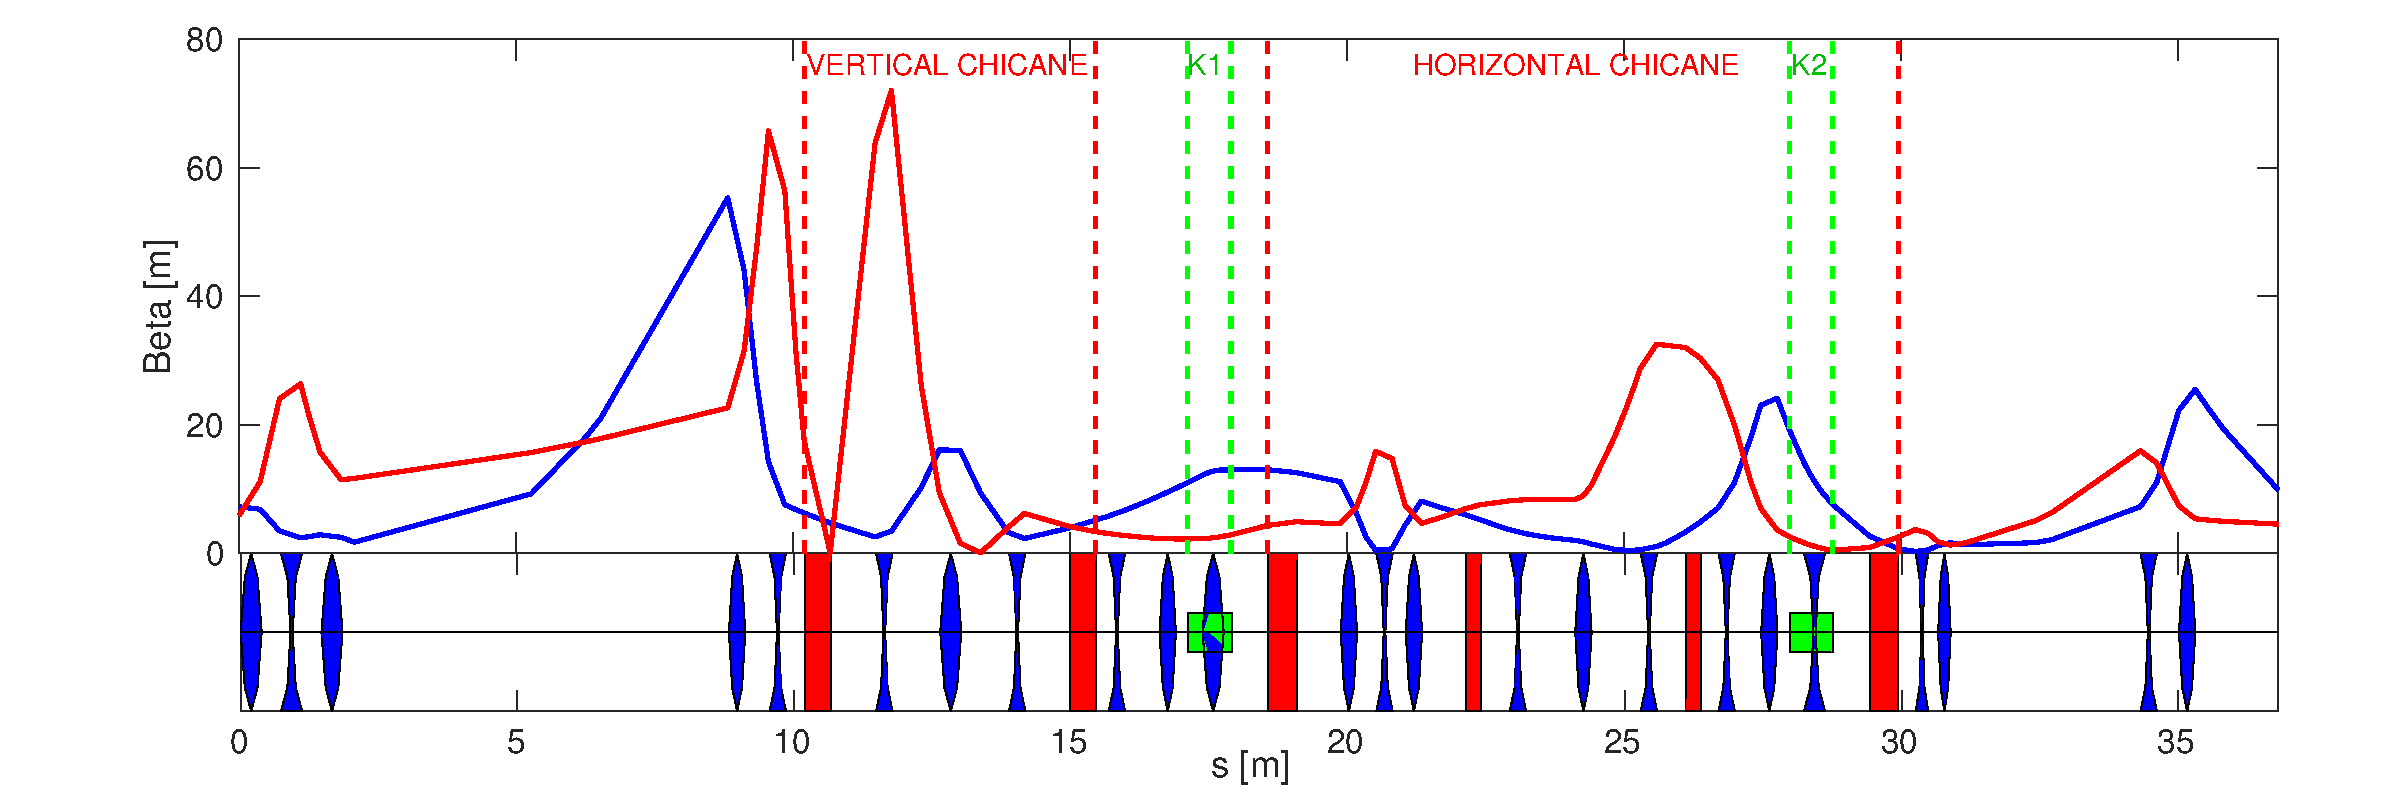
\includegraphics[width=0.75\hsize]{Figures/optics/pffOpticsBeta}
  \caption{Horizontal (blue) and vertical (red) beta functions in the new TL2 optics. Blue convex lenses indicate focusing quadrupoles and blue concave lenses defocusing quadrupoles. Red rectangles mark the position of dipoles, and green squares the
position of the two PFF kickers.}
  \label{f:pffOpticsBeta}
  \centering
  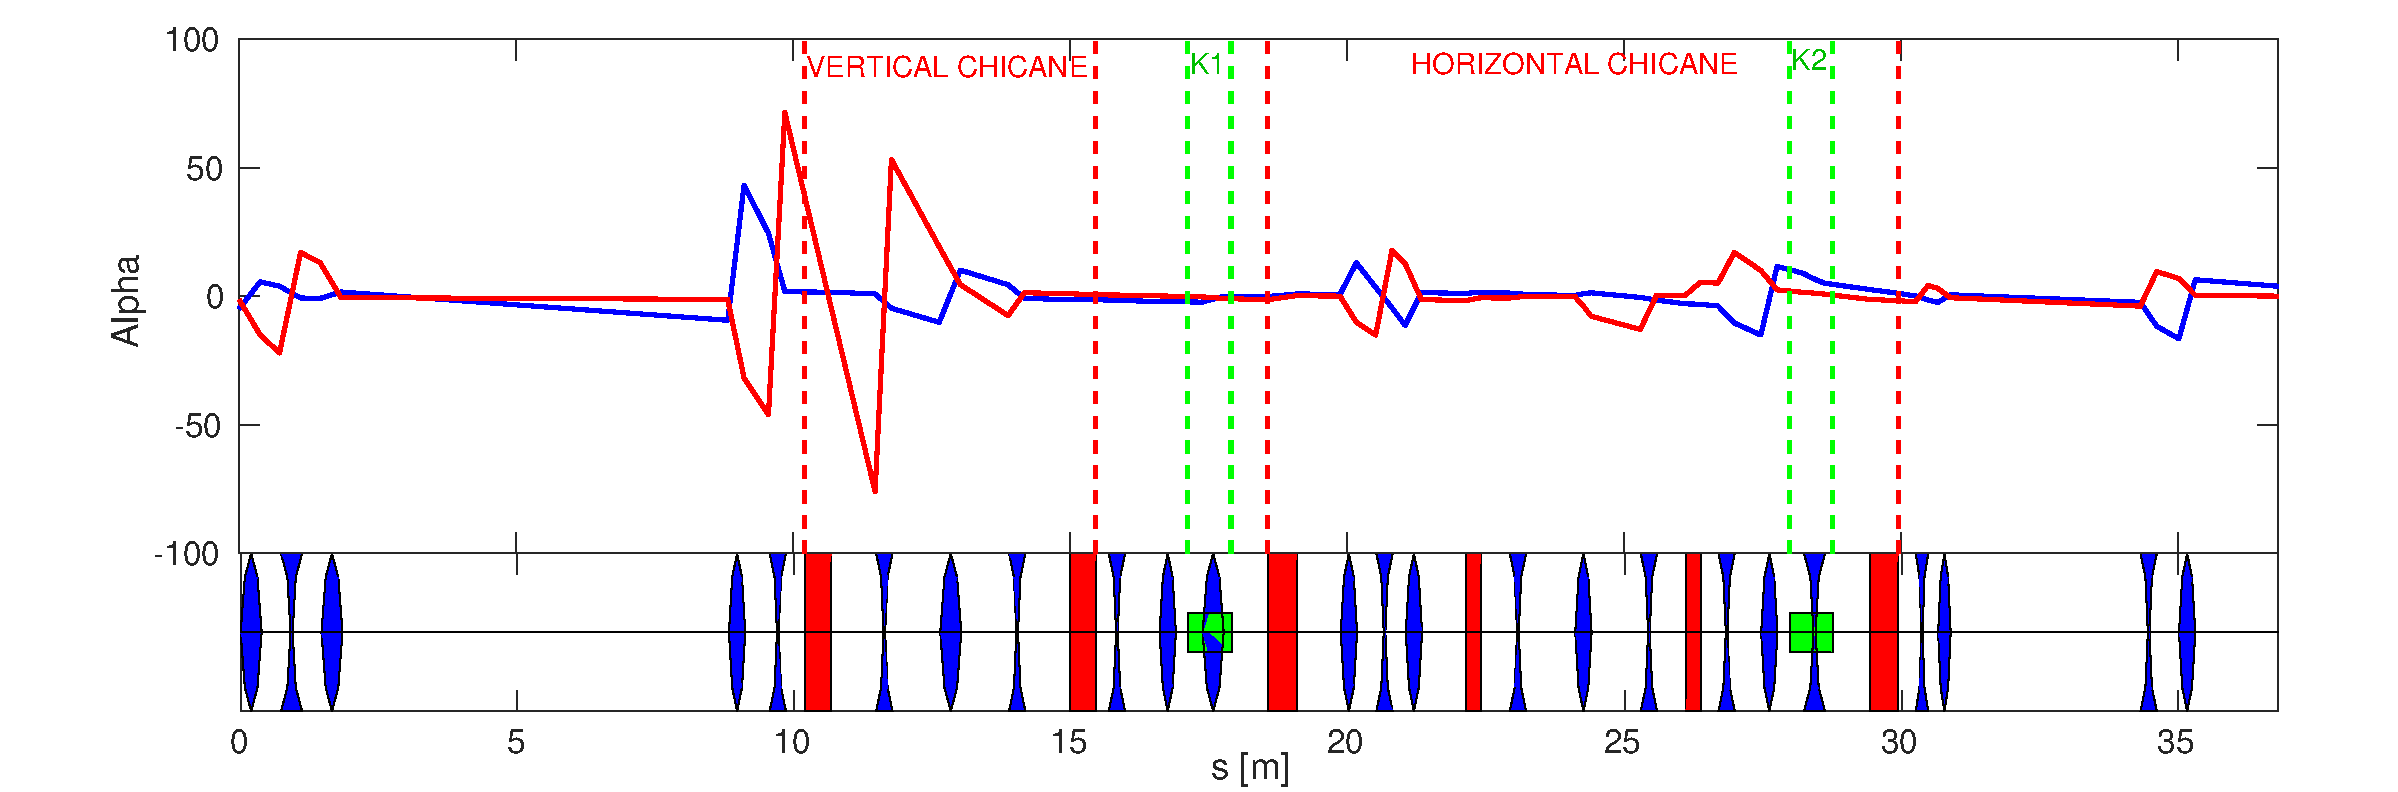
\includegraphics[width=0.75\hsize]{Figures/optics/pffOpticsAlpha}
  \caption{Horizontal (blue) and vertical (red) alpha functions in the new TL2 optics. Blue convex lenses indicate focusing quadrupoles and blue concave lenses defocusing quadrupoles. Red rectangles mark the position of dipoles, and green squares the position of the two PFF kickers.}
  \label{f:pffOpticsAlpha}
\end{figure}

\begin{figure}
  \centering
   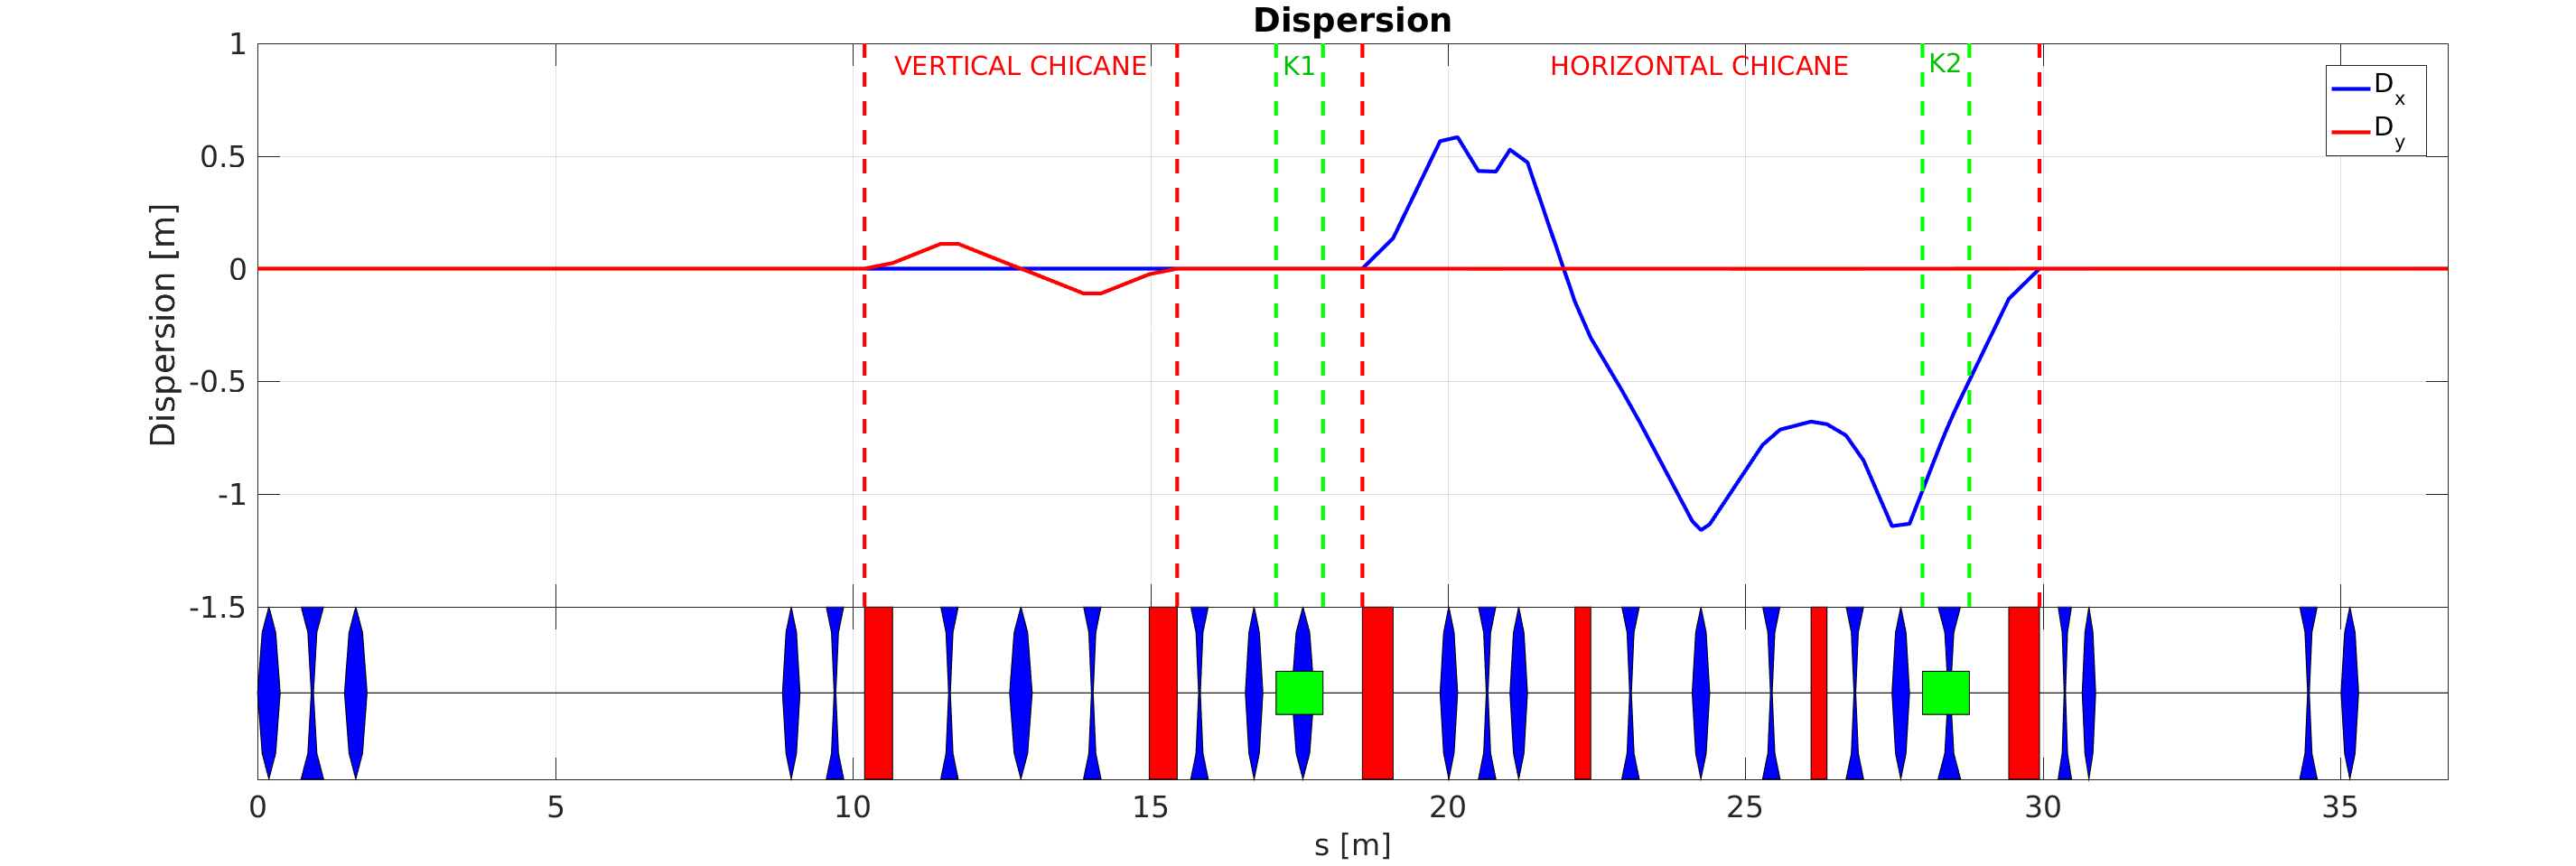
\includegraphics[width=0.75\hsize]{Figures/optics/pffOpticsDisp}
  \caption{Horizontal (blue) and vertical (red) dispersion in the new TL2 optics. Blue convex lenses indicate focusing quadrupoles and blue concave lenses defocusing quadrupoles. Red rectangles mark the position of dipoles, and green squares the position of the two PFF kickers.}
  \label{f:pffOpticsDisp}
  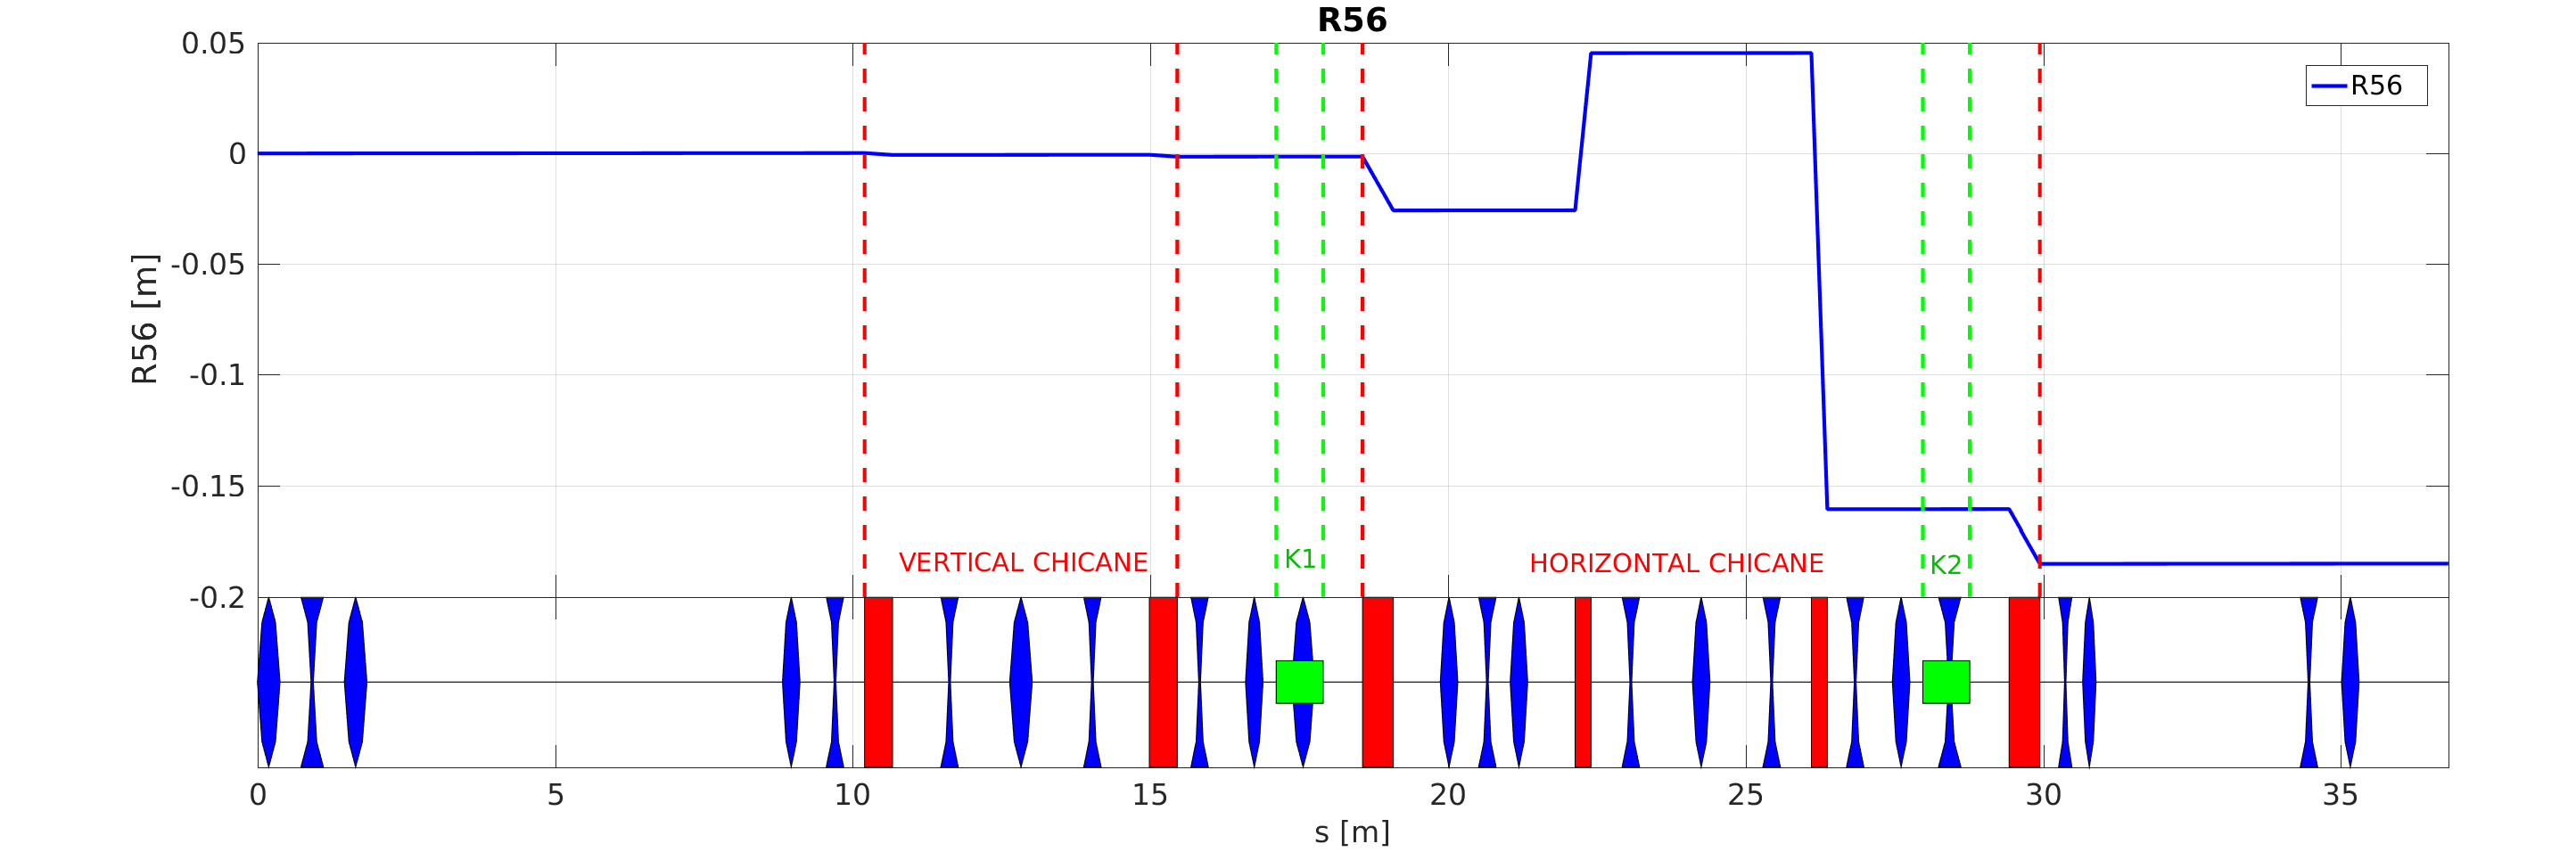
\includegraphics[width=0.75\hsize]{Figures/optics/pffOpticsR56}
  \caption{\(R_{56}\) in the new TL2 optics. Blue convex lenses indicate focusing quadrupoles and blue concave lenses defocusing quadrupoles. Red rectangles mark the position of dipoles, and green squares the position of the two PFF kickers.}
  \label{f:pffOpticsR56}
\end{figure}

\begin{figure}
  \centering
  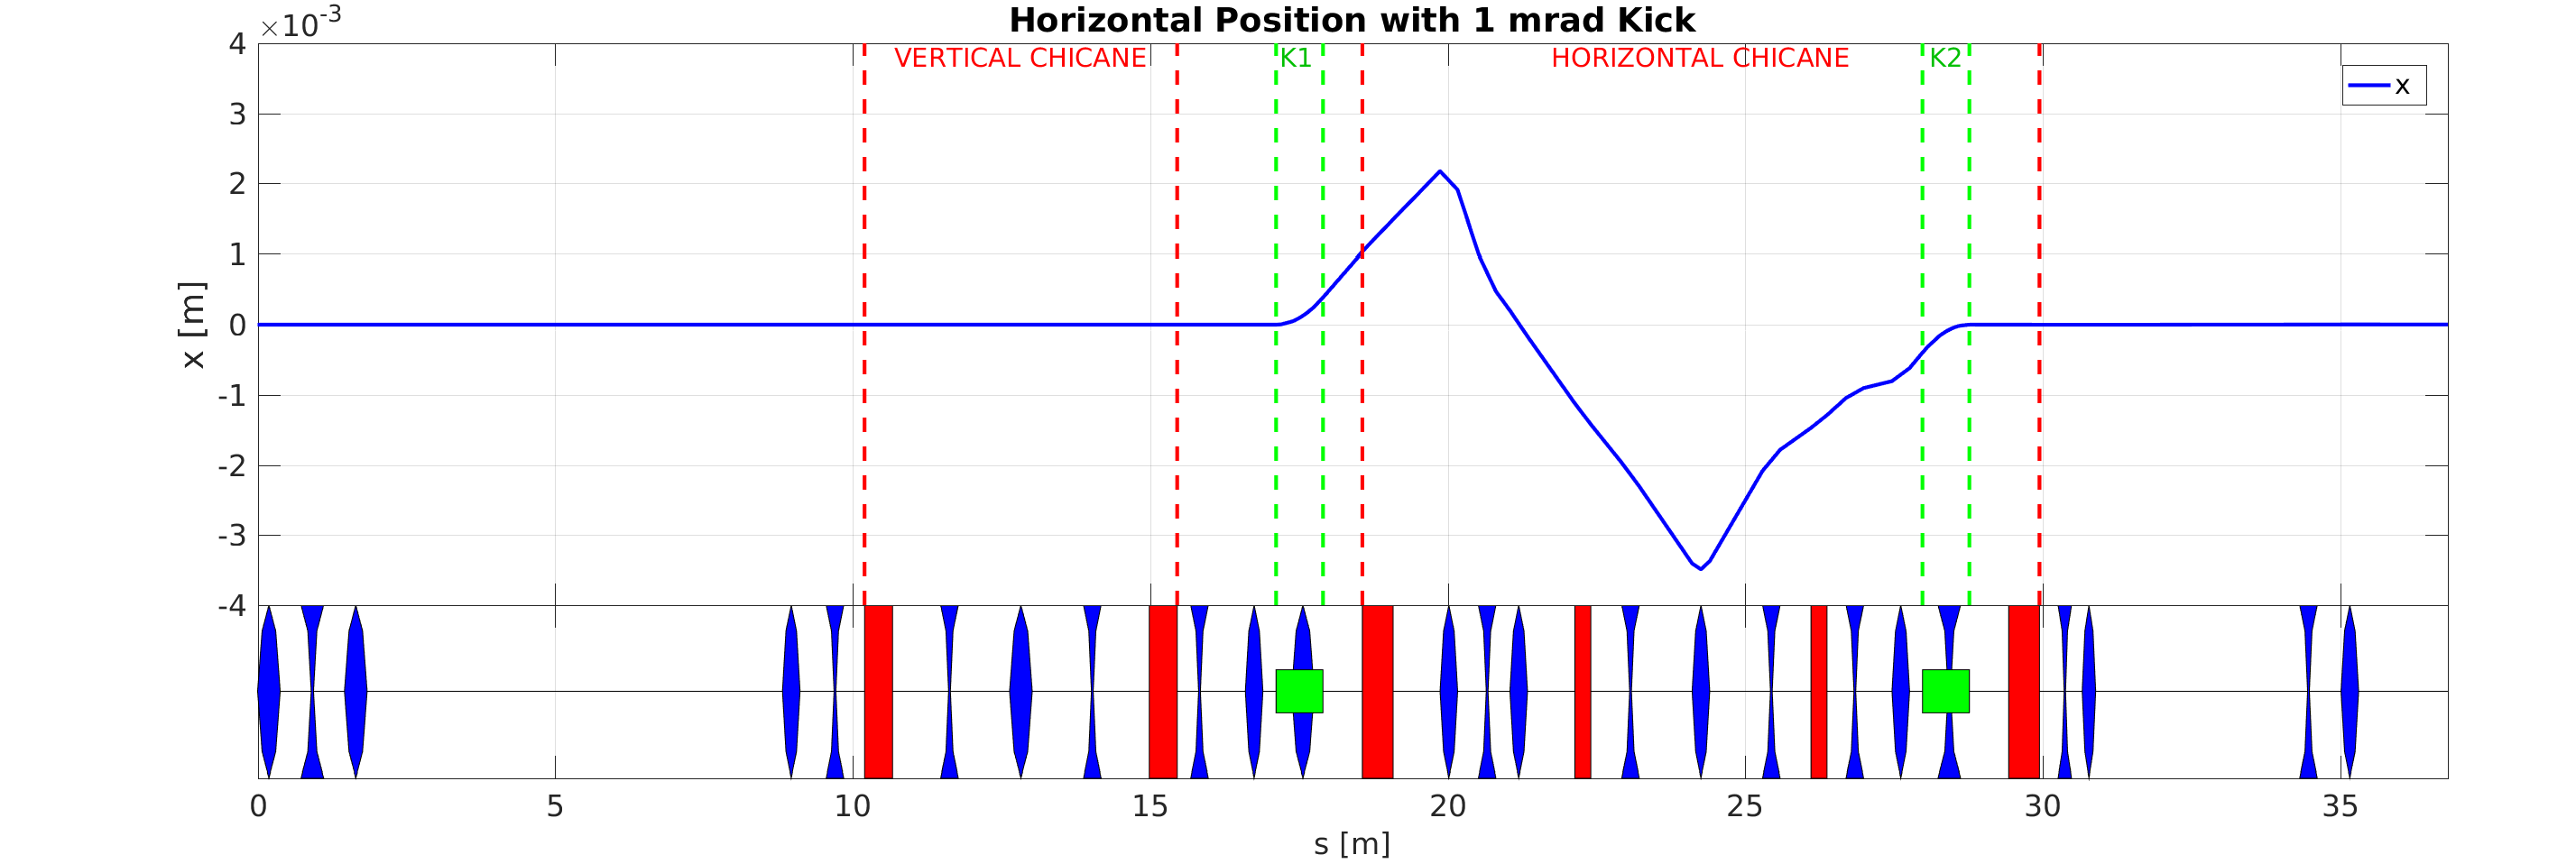
\includegraphics[width=0.75\hsize]{Figures/optics/pffOpticsX}
  \caption{Horizontal orbit in the TL2 chicane with a 1~mrad kick from the PFF kickers. Blue convex lenses indicate focusing quadrupoles and blue concave lenses defocusing quadrupoles. Red rectangles mark the position of dipoles, and green squares the position of the two PFF kickers.}
  \label{f:pffOpticsX}
  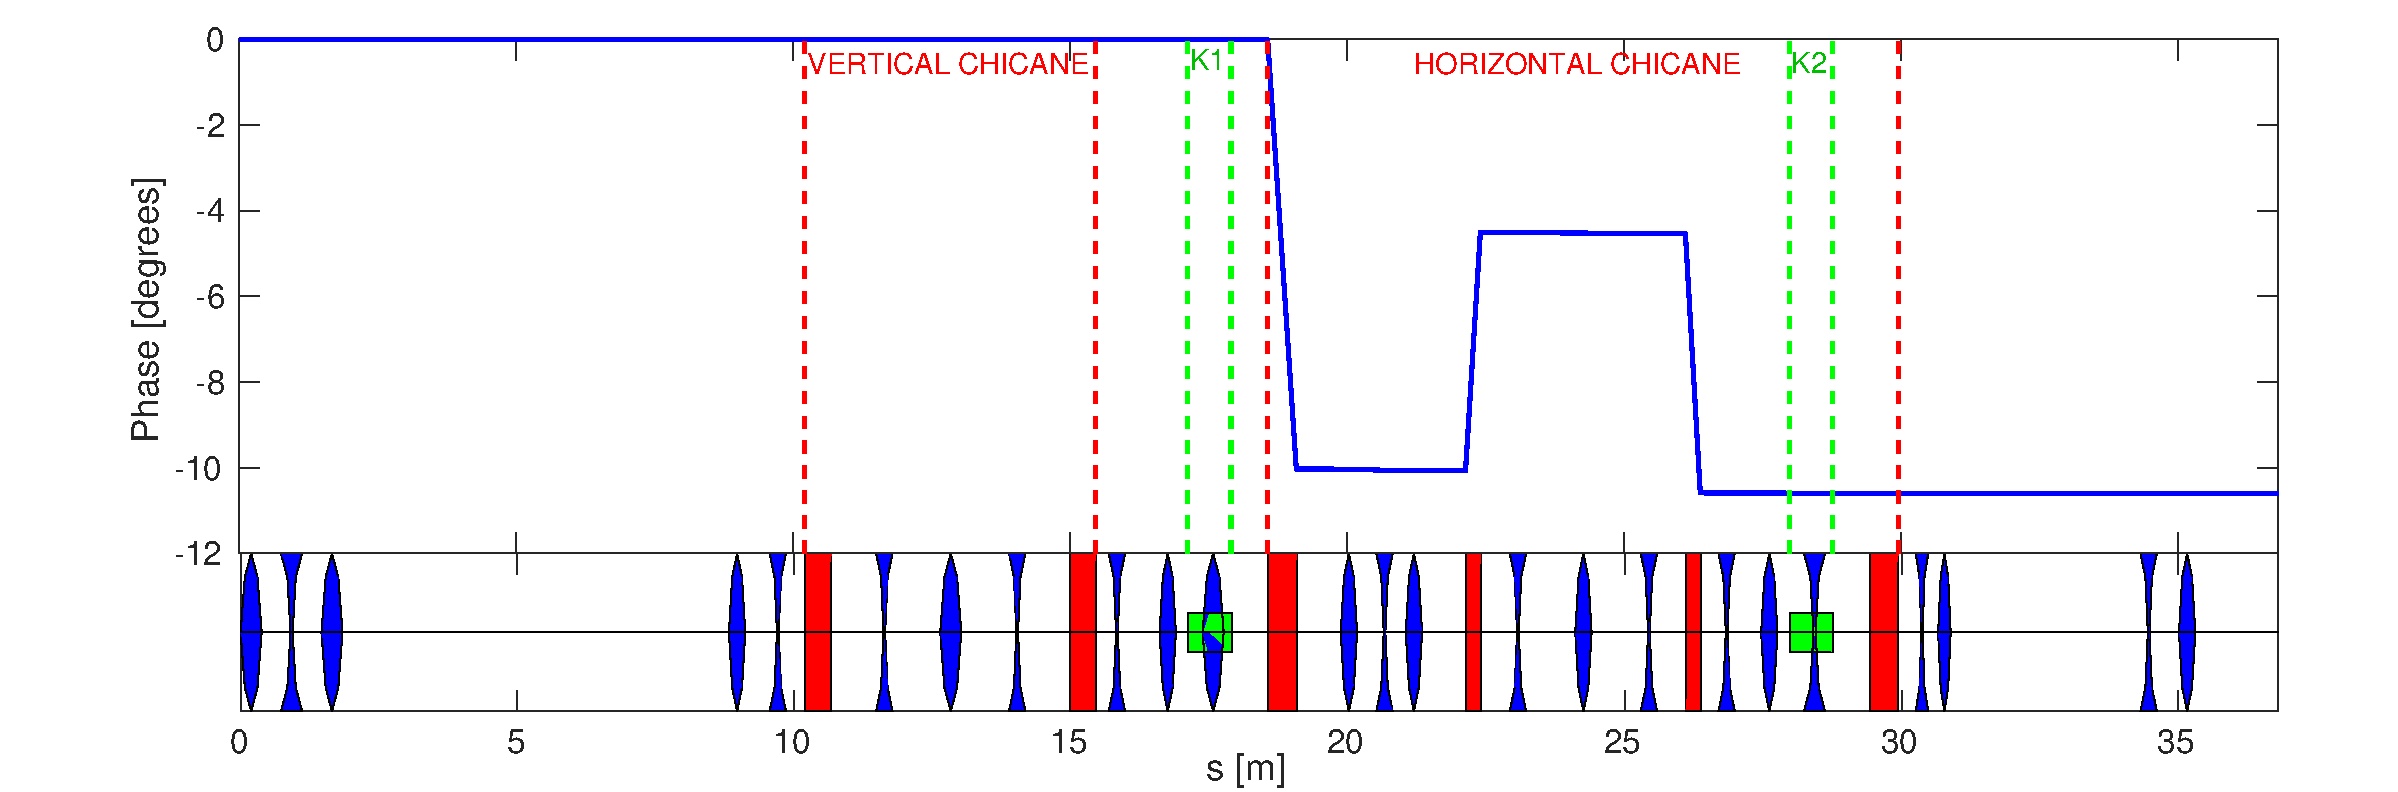
\includegraphics[width=0.75\hsize]{Figures/optics/pffOpticsPhase}
  \caption{Phase in the TL2 chicane with a 1~mrad kick from the PFF kickers. Blue convex lenses indicate focusing quadrupoles and blue concave lenses defocusing quadrupoles. Red rectangles mark the position of dipoles, and green squares the position of the two PFF kickers.}
  \label{f:pffOpticsPhase}
\end{figure}
\end{landscape}}